\documentclass[pdftex,12pt,a4paper]{report}

%------------------------------------------------
%	PACKAGES
%------------------------------------------------

\usepackage{webis}

\usepackage{mwe}

\usepackage{ucs}

\usepackage[utf8x]{inputenc}

\usepackage{ngerman}

\usepackage[gen]{eurosym}

%\usepackage{hyperref}

\usepackage{url}

\usepackage{enumitem}

\usepackage{amsmath}

\usepackage{algorithm}

\usepackage{algpseudocode}

\usepackage{array}

\usepackage{mathtools}

%------------------------------------------------
%	DEFINE AND CONFIGURE ENVIRONMENTS
%------------------------------------------------

% Figure (Latex definition)
\usepackage[font=small,labelfont=bf,width=12cm]{caption}
\usepackage{chngcntr}
\counterwithout{figure}{chapter} 

% Anforderung (Own definition)
\newtheorem{anforderung}{Anforderung}[section]
\counterwithout{anforderung}{section}

% Hypothese (Own definition)
\newtheorem{hypothese}{Hypothese}[section]
\counterwithout{hypothese}{section}


%------------------------------------------------
%	CONFIGURATION FOR COVER PAGE
%------------------------------------------------

\global\arbeit{Bachelorarbeit}

\global\titel{Echtzeit Hinderniserkennung für unbemannte Flugsysteme unter Benutzung eines Stereo Kamera Systems}

\global\subtitel{}

\global\bearbeiter{Hagen Hiller}

\global\betreuer{Dr. Jens Kersten}

\global\erstgutachter{Prof. Dr. Volker Rodehorst}

\global\zweitgutachter{TBA} % TODO Zweitkorrektor

\global\abgabetermin{25.01.2016}

\global\ort{Weimar}

\global\matrikelnummer{110514}

\global\geburtsdatum{04.06.1992}

\global\geburtsort{Berlin}

%------------------------------------------------
%	START DOCUMENT
%------------------------------------------------

\begin{document}

%------------------------------------------------
%	COVER PAGE
%------------------------------------------------

\deckblatt

%------------------------------------------------
%	DECLARATION FOR EXAMINATION OFFICE
%------------------------------------------------

\erklaerung

%------------------------------------------------
%	ABSTRACT
%------------------------------------------------

\begin{abstract}

Lorem ipsum dolor sit Amet.

\end{abstract}


%------------------------------------------------
%	TABLE OF CONTENTS
%------------------------------------------------

\tableofcontents

%------------------------------------------------
%	THESIS CHAPTERS
%------------------------------------------------

\chapter{Einführung}
\label{chp:introduction}
\section{Motivation}
\label{sec:motivation}

Die vorliegende Arbeit ist im Forschungsgebiet Robotik angesiedelt und behandelt bildbasierte Verfahren zur Erkennung von Hindernissen für autonome Flugsysteme (UAV \footnote{Unmanned Aircraft System}). Diese Verfahren sind für die Navigation sowie für die autonome Erkundung von unbekannten oder unzugänglichen Gebieten unerlässlich. Dabei müssen nicht nur die physikalischen Eigenschaften der Drohne betrachtet werden sondern auch die Fusion verschiedenster Sensoren.\\

\noindent
Ein wichtiges Kriterium in der Entwicklung autonomer Roboter ist die Erkennung von Hindernissen in Echtzeit. Dabei muss jedoch zuerst definiert werden was vom System als potentielles Hindernis erkannt werden soll. Prinzipiell sind alle Objekte welche sich in der unmittelbaren Nähe des Systems befinden eine Gefahrenquelle. Im Fall eines Kamera-basierten Systems mit lediglich einer Hauptblickrichtung, ist die Detektion jedoch beschränkt, so dass eine Einschränkung der zugelassenen Manöver, z.B. auf eine Bewegung lediglich in Blickrichtung der Kamera, erfolgen sollte. Dies schließt eine Kollision mit Objektn außerhalb des Sichtfeldes aus. Auch sehr weit entfernte Objekte sind prinzipiell nicht als Hindernis anzusehen, wobei die maximal zu betrachtende Gefahrendistanz abhängig von der aktuellen Bewegungsgeschwindigkeit angepasst werden sollte. Unter Betrachtung dieser Gesichtspunkte wird ein Hindernis innerhalb dieser Arbeit als ein Objekt definiert welches sich innerhalb eines definierten Distanzbereichs und innerhalb des Sichtfeldes der Kamera befindet.\\

\noindent
Die hauptsächliche Anwendung des im Rahmen dieser Arbeit entwickelten Systems zielt auf die autonome Navigation von Unbemannten Flugsystemen ab. Weitere Anwendungsbereiche können sowohl komplexerer als auch einfacherer Natur sein. Prinzipiell ist es möglich die entwickelten Algorithmen und Methoden im Automobil Bereich zu verwenden um beispielsweise Objekte vor oder Hinter dem Kraftfahrzeug zu erkennen und die Distanz zu berechnen. 

% TODO neues Beispiel
%Weiterhin ist es vorstellbar grobe kartographische Höhen Klassifikationen vorzunehmen, um Bild basiert eine Höhenkarte geographischer Areale zu erstellen. Das jeweilige Anwendungsszenario richtet sich jedoch dabei nach der verwendeten Hardware. 

\section{Hardwarekomponenten}
\label{sec:setup}

% TODO Einleitung siehe Jens version
Die aktive Entwicklung der Methoden und Algorithmen erfolgte im Hinblick auf eine Verwendung dieser durch das von Ascending Technologies \cite{asctec} entwickelte UAS Pelican (Abbildung \ref{img:pelican}).
Es handelt sich dabei um einen Quadrocopter der speziell für Forschungszwecke entwickelt wurde. Er ist mit einem Bordcomputer ausgestattet, der die nötige Leistung für die Entwicklung der Algorithmen bereitstellt (3rd Generation Intel Core i7). Weiterhin wurden zwei MatrixVision BlueFOX mv-MLC200wC Industriekameras \cite{matrixvision} als visuelles System verwendet. Die maximale Auflösung beider Kameras beträgt $752\times480$ bei 60 möglichen Bildern pro Sekunde, in Abhängigkeit verschiedener Parameter (verwendetet Verschlusszeit, aufgenommene Bitrate, u. a). Für den Echtzeit-Aspekt des Systems werden beide Kameras in einem horizontalen und vertikalen Binning-Modus verwendet. Dies halbiert die Anzahl der Bildpunkte in beiden Dimensionen auf $376\times240$, wodurch der Berechnungsaufwand verringert und die die Aufnahmerate der Kameras auf bis zu 170 Einzelbilder pro Sekunde maximiert wird.
\noindent
Für die Implementierung der Algorithmen wurde die freie Computer Vision Bibliothek OpenCV \cite{opencv} verwendet. Diese stellt benötigte algebraische Grundoperationen sowie bestimmte Algorithmen, welche im Rahmen dieser Arbeit genutzt wurden, zur Verfügung.
	% TODO Setup erweitern --> mehr?!
\begin{figure}[h]
	\centering
	\begin{tabular}{cc}
	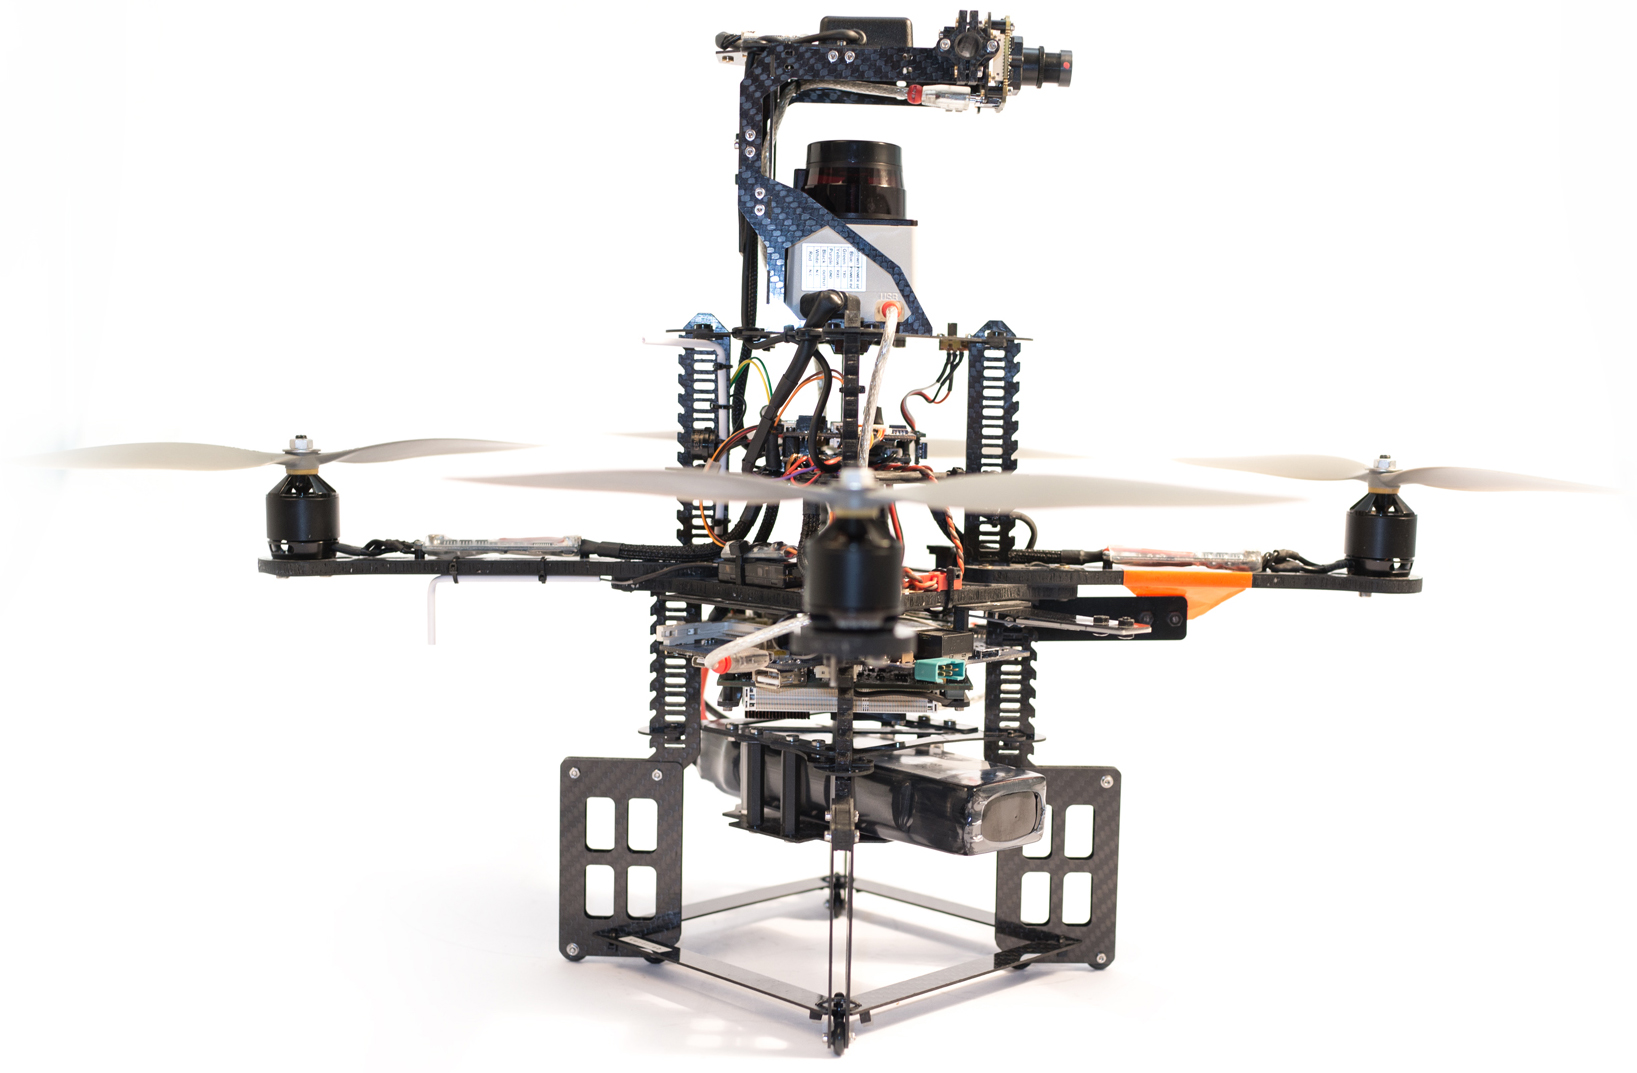
\includegraphics[width=6cm]{img/pelican} &
	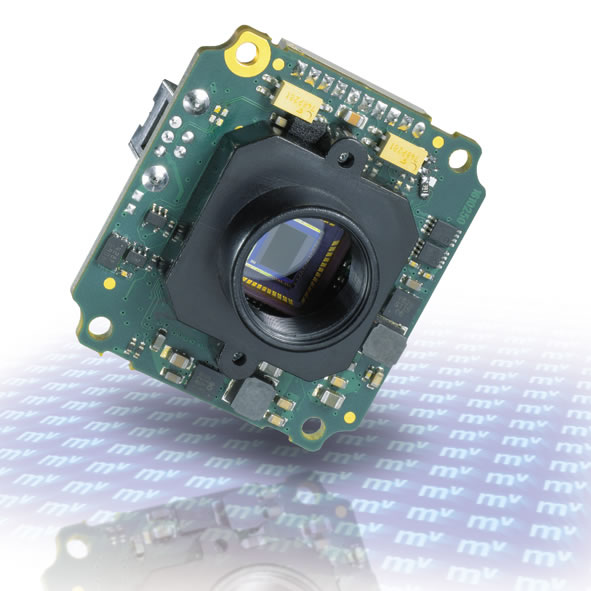
\includegraphics[width=6cm]{img/camera}
	\end{tabular}
	\caption{AscTec Pelika (links), MatrixVision BlueFOX mv-MLC200wC (rechts)}
	\label{img:pelican}
\end{figure}


\section{Ziel der Arbeit}
\label{sec:ziel_der_arbeit}
Basierend auf photogrammetrischen Konzepten ist es möglich, räumliche Tiefe aus zweidimensionalen Bilddaten zu berechnen. Generell werden mindestens zwei Bilder aus unterschiedlichen Standpunkten für die Berechnung dreidimensionaler Informationen benötigt. Das daraus resultierende Problem welches bei der Benutzung einer Kamera entsteht ist die oft ungenau Schätzung der relativen Orientierung sowie die damit einher gehende Skalierung. Bei der Verwendung eines Stereosystems ist die relative Orientierung beider Kameras zueinander bereits bekannt, was eine direkte Berechnung metrischer Koordinaten ermöglicht. Da Zuverlässigkeit sowie Genauigkeit vor allem im Kontext der Navigation in Innenräumen sehr wichtig ist wurde in dieser Arbeit auf ein Stereo-Setup gesetzt.
% TODO nochmal rüber lesen

%Unter Betrachtung dieser Techniken wurde im Rahmen dieser Arbeit \\

\noindent
Vor diesem Hintergrund werden zunächst einige State of the Art Methoden der Hinderniserkennung beschrieben wobei dabei zwischen aktiven und passiven optischen Systemen unterschieden wird. Diese Einteilung dient einerseits dafür einen Überblick über bereits bestehende Techniken sowie implementierte Systeme zu erhalten, andererseits um auch die Vor- und Nachteile der jeweiligen Technik herauszuarbeiten. Kapitel \ref{chp:concepts} behandelt die dieser Arbeit zugrundeliegenden Konzepte und Algorithmen. Des Weiteren wird das im Rahmen dieser Arbeit implementierte Framework sowie dessen Funktionsweise erläutert. Im Anschluss daran beschreibt Kapitel \ref{chp:developed_algorithms} die beiden entwickelten Methoden zur bildbasierten Hinderniserkennung und deren Implementierung detailliert. Anschließend erfolgt die Evaluation beider Verfahren unter den Gesichtspunkten Robustheit sowie der Performance. 
% TODO beschreiben was mit dem letzten satz
Weitere Tests zur zukünftigen Verbesserung der Algorithmen weisen auf welches aktuellen Limitierungen durch einerseits genutzte Konzepte vorliegen. Kapitel \ref{chp:conflicts} erläutert eben diese Limitierungen und gibt Ansätze zur Lösung aus der Fachliteratur sowie eigene Konzepte zur Bewältigung dieser. Die anschliessende Diskussion wertet die im Rahmen der Evaluation in Kapitel \ref{chp:evaluation} erlangten Ergebnisse weitergehend aus und stellt beide Algorithmen gegenüber. Kapitel \ref{chp:fazit} zieht ein Ré­su­mé aus den Ergebnissen der Arbeit und gibt einen Ausblick auf mögliche zukünftige Arbeiten in diesem Bereich.

%------------------------------------------------

\chapter{Anforderungsanalyse}
\label{chp:anforderungsanalyse}
Lorem ipsum dolor sit amet.

% ---------------------- section -----------------------
\section{Bildaufnahme und Preprocessing}
\label{sec:bildaufnahme_preprocessing}

	\begin{anforderung}
	\label{req:bildaufnahme}
		Die zur Erkennung von Hindernissen verwendeten Bilder müssen kalibriert, entzerrt sowie stereo-rektifiziert vorliegen.
	\end{anforderung}

\noindent
Um Anforderung \ref{req:bildaufnahme} zu erfüllen müssen zunächst die intrinsischen und extrinsischen Parameter der Kamera berechnet werden. Dieser Prozess wird als Kalibierung der Kamera bezeichnet. Dafür werden Bilder eines Kalibierobjektes aufgenommen. Diese sind meistens einfache Schachbrettmuster mit ungleicher Anzahl an Quadraten, oder auch radiale Objekte mit einem spezifischerem Aufbau. Der Prozess der Kalibierung zielt darauf ab die 'inneren' Parameter der Kamera zu bestimmen. Dies beinhaltet einerseits die Kameramatrix in welcher Parameter wie der Fokus Punkt(Focal Point), der Bildhauptpunkt(Principal Point) sowie die Brennweite der der Kamera. Weiterhin werden geometrische Verzerrungen des Bildes,  parametrisiert und somit nutzbar für die Entzerrung der Bilder in weiteren Schritten. Weiterhin werden bei der Kallibrierung die extrinsischen (äußeren) Parameter der Kamera bestimmt. Zu diesen zählt die Translation (x,y und z) sowie die Rotation der Kamera um die jeweiligen Achsen des Weltkoordinatensystems. Ein spezieller Aspekt bei der Kalibierung von Stereo-Systemen ist die Berechnung der extrinsischen Parameter von einer Kamera zur anderen. Die dabei berechnete Translation einer Kamera zur Referenzkamera wird als Baseline bezeichnet. Diese ist für Prozeduren wie Stereo-Matching unabdingbar. Der Prozess der Parameterfindung ist in der Regel ein Prozess welcher einmalig nach dem Aufbau ausgeführt werden muss und solange währt wie sich nichts am Aufbau der Kameras ändert (Objektive, Translation, Rotation).\\

\noindent
Folgend aus der Kalibrierung der Kameras beginnt der Prozess der Rektifizierung der Bilder. Dieser kann dabei in zwei Schritte unterteilt werden, einerseits die Berechung der Region of Interest, andererseits die Rektifizierung jedes aufgenommenen Einzelbildes. Mithilfe der zuvor berechneten intrinsischen und extrinsischen Parameter kann nun die Transformation der beiden Kamerabilder zueinander berechnet werden. Dies geschieht unter dem Aspekt der Epipolargeometrie. Nach der Rektifizierung und dem Anwenden der ROIs auf beiden Kamerabildern entspricht die jeweilige Pixelreihe im linken Bild der Pixelreihe mit dem selben Index im rechten Bild.\\
    % TODO retification beschreiben

% ---------------------- section -----------------------
\section{Performanz}
\label{sec:performanz}

	\begin{anforderung}
	\label{req:performanz}
		Das System sollte Hindernisse in Echtzeit erfassen und erkennen können.
	\end{anforderung}


% ---------------------- section -----------------------
\section{Erfassung von Hindernissen}
\label{sec:erfassung_von_hindernissen}

	\begin{anforderung}
	\label{req:erfassung_von_hindernissen}
		Die Erfassung von Hindernissen sollte eine signifikant hohe Wahrscheinlichkeit haben um etwaige Fehlentscheidungen zu vermeiden.
	\end{anforderung}
	

% ---------------------- section -----------------------
\section{Positionsinformationen}
\label{sec:positionsinformationen}

	\begin{anforderung}
	\label{req:positionsinformationen}
		Relative Positionen der gefundenen Objekte müssen in jedem Frame vorliegen.
	\end{anforderung}


%------------------------------------------------

\chapter{State of the Art Algorithmen}
\label{chp:stateoftheart}
Ein aktuell erforschtes Feld in der Entwicklung autonomer Systeme ist die Vermeidung von Hindernissen in Echtzeit. Die wesentliche Grundlage dafür besteht in der Erkennung der Hindernisse. Dies geschieht oft mit Hilfe optischer Messtechniken.\\

\noindent
Im folgenden Kapitel werden einige State of the Art Verfahren erläutert. Dabei werden zunächst verschiedene aktive optische Systeme näher beschrieben, bei denen die betrachtete Szene aktiv ausgeleuchtet wird. Anschließend erfolgt die Analyse weiterer passiver optischer Algorithmen, welche auf der Berechnung von sogenannten Disparitätenkarten unter Zuhilfenahme Stereo-optischer Systeme basiert. Diese berechneten Tiefenkarten enthalten die horizontale Verschiebung korrespondierender Bereiche in beiden Bildern. Die Kalkulation solcher ist generell sehr rechenaufwändig, liefert aber nach der Auswertung Informationen über die Entfernung sowie Position der abgebildeten Szene. Die dabei erhaltenen Ergebnisse hängen von dem jeweils verwendeten \emph{Stereo-Matching} Algorithmus ab.

% ---------------------- section -----------------------
\section{Aktiv optische Algorithmen}
\label{sec:kamera_basierte_he}
% ToDo: quellen aktiv optische algorithmen
Aktiv optische Algorithmen basieren auf einer aktiven Beleuchtung der zu rekonstruierenden Szene. Dies geschieht indem beispielsweise Muster auf die Szene projiziert werden (Gitter, Streifen, Farben, etc.), mit deren Hilfe es möglich ist, das Korrespondenzproblem, also das finden korrespondierender Punkte in zwei Bildern, einfach und robust zu lösen. Uniforme bzw. einfache Muster führen zu Mehrdeutigkeiten, die leicht Fehlzuordnungen herbeiführen können. Ein alternativer Ansatz ist die Projektion zufälliger Muster, um etwaige falsche Korrespondenzen durch bewusste Zufälligkeit zu vermeiden. Ein weiteres Feld in der Betrachtung aktiver visueller Techniken ist \emph{Time of Flight} (TOF). Hierbei wird die Szene mit einem Lichtimpuls (meist infrarot) ausgeleuchtet und für jeden Pixel die Zeit gemessen, die jener benötigt, um wieder auf dem Sensor aufzutreffen. Damit ist es möglich, in geringer Auflösung dichte Tiefendaten für jedes Einzelbild zu messen.\\

\noindent
Die von Lee et al. \cite{lee2012intelligent} vorgeschlagene Methodik der Hinderniserkennung bedient sich einer TOF Kamera. Die aufgenommenen Tiefenbilder werden basierend auf den Tiefenmessungen segmentiert. Dabei werden mi Hilfe eines Algorithmus zur Kantenerkennung jene herausgefiltert und anschliessend von der Tiefenkarte subtrahiert, um diese in weiteren Schritten als einzelne Objekte betrachten zu können. Anschließend erfolgt eine Tiefenanalyse der nun vorliegenden einzelnen Segmente. Um die gefundenen Segmente als Hindernis klassifizieren zu können wird zunächst die Standardabweichung der Disparität jedes Segements berechnet. Da die Tiefenwerte des Bodens einen hohen Grad der Streuung aufweisen ist die Standardabweichung dessen höher als bei anderen Segmenten. Diese Information dient zur Unterscheidung zwischen Hindernis und Boden. Dabei gelten Hindernisse als sich bewegende oder statische Objekte, welche sich innerhalb eines definierten Gefahrenbereichs befinden. Lee et al. definieren Ihre Gefahrenzone dabei mit $1-2$ Metern. Die erkannten Hindernisse werden nun anhand der mittleren Distanz des Segmentes markiert.\\

\noindent
Bei der Entwicklung eines autonomen Roboters zur Indoor-Überwachung verschiedener Areale bedienen sich Correa et al. \cite{correa2012mobile} eines Microsoft Kinect Sensors zur Erstellung von Disparitätenkarten nach dem \emph{Time of Flight} Prinzip. Dabei werden diese in mehrere horizontale Segmente eingeteilt. Die finale Karte besteht aus 5 Bereichen, von denen 3 als mögliche Richtungen betrachtet werden. Sobald die die minimalste Distanz eines Sektors geringer als 60 cm ist wird angenommen, dass sich das System vor einem Hindernis befindet. Ausgehend von der Menge an Sektoren mit gefunden Hindernissen wird die neue Bewegungsrichtung angepasst.

% ---------------------- section -----------------------
\section{Passiv optische Algorithmen}
\label{sec:sensor_basierte_he}
% ToDo: quellen passiv optische algorithmen
Passiv optische Algorithmen beziehen sich auf die Berechnung dreidimensionaler Informationen aus Bildern ohne eigene Lichtquelle. Dabei sind viele dieser Methoden an das menschliche oder auch tierische Sehen angelehnt. Viele Ansätze nutzen das \emph{Stereo Vision} Prinzip  welches durch die Differenz zweier Bilder derselben Szene einen Eindruck von Tiefe verschafft. Weiterhin kann eine dreidimensionale Rekonstruktion der Umgebung durch die Analyse von Bildern hinsichtlich Lichteinflüssen, Schattierungen oder durch Veränderung des Kamerafokus vorgenommen werden.\\

\noindent
Bei der Entwicklung eines autonomen Roboters auf Bodenebene werden nach Kostavelis et al, \cite{kostavelis2010comparative} die errechneten Disparitätenkarten in 3 gleich große horizontale Bildbereiche aufgeteilt, welche die möglichen Bewegungsrichtungen des Systems repräsentieren. Für jedes dieser einzelnen Unterbilder wird nun der Durchschnitt der Disparitäten berechnet, wobei der Bildteil mit dem geringsten Wert auf Hindernisse hinweist, welche sich näher am System befinden. Angesichts der Tatsache, dass die Entscheidung darüber, welcher Weg als der sicherste angesehen werden muß, teilweise schwer zu treffen ist, wurde die sogenannte \emph{threshold estimation} Methode entwickelt. Die Unterteilung der Bilder wird hier ebenfalls in drei Regionen vorgenommen. Zunächst werden alle Pixel deren Werte sich über einem vordefinierten Schwellwert befinden markiert und gezählt. Wenn die Anzahl der als Hindernis definierten Pixel über einem ebenfalls vordefinierten Prozentsatz liegen, so wird ein Hindernis als gefunden markiert (in der jeweiligen Region). Die letzte vorgestellte Methode von Kostavelis et al. orientiert sich in ihrer Funktionsweise an der soeben beschriebenen Schwellwertschätzung und erweitert den Algorithmus um die Betrachtung aller 3 Bildteile. Bei der \emph{multi threshold estimation} wird jedes Drittel des Bildes betrachtetet, wobei in allen Regionen nach Pixeln innerhalb des Schwellwerts gesucht und diese markiert werden. Anschließend werden die Ergebnisse untereinander verglichen, und das Drittel mit dem geringsten Wert als Hindernis ausgewählt. Sollten die prozentualen Werte aller Drittel größer sein als die gegebene Grenze so wird angenommen das sich das Hindernis sehr nah vor dem System befindet.\\

\noindent
Eine weitere Methode zur Hindernisvermeidung für UAS wurde von Richards et al. \cite{richards2014obstacle} vorgestellt. Optischer Fluss sowie \emph{Feature Tracking} bieten dabei die Grundlage für die Erkennung, Vermeidung und Voraussage, welcher Bereich im Raum der sicherste ist. Dabei gehen die beiden Ausgangstechniken jeweils einer anderen Aufgabe nach. Der Optische Fluss dient zum Erkennen und Verfolgen von Objekten sowie für die Voraussage der Position im nächsten Einzelbild, wohingegen das \emph{Feature Tracking} \cite{shi1994good} für die Erkennung von markanten Punkten innerhalb des Objektes genutzt wird. Bei diesem wird in jedem folgenden Einzelbild verglichen, ob bereits bekannte Punkte innerhalb einer bestimmten Distanz mit denen des aktuellen Bildes übereinstimmen. Zur Schätzung zu erwartenden Position der Merkmale im darauffolgenden Bild werden mit Hilfe des Optische Fluss’ die Verschiebungsvektoren zwischen beiden Bildern berechnet. Aufgrund dessen, dass der zugrunde liegende Algorithmus von Lukas-Kanade \cite{lucas1981iterative} nur bei kleinen Verschiebungen valide Ergebnisse liefert, wird ein pyramidaler Ansatz \cite{bouguet2001pyramidal} für das Matching verwendet, bei welchem beide Bilder eines \emph{frames} herunter skaliert werden. Durch die Verbindung dieser beiden Techniken lassen sich Objekte erkennen und verfolgen. Zur Bestimmung der nächstbesten Position für das UAV wird ausgehend von den berechneten Resultaten (gefundene und erkannte Hindernisse) eine stochastische Matrix erstellt welche zur weiteren Planung des Fluges verwendet wird.\\

\noindent
Bei der Entwicklung von Algorithmen, welche auf räumlicher Tiefe basieren, bieten stereo-optische Systeme einen großen Vorteil. Durch den Versatz der Kameras auf der Basislinie wird die Szene aus zwei minimal verschiedenen Blickwinkeln aufgenommen. Dies ermöglicht die Berechnung dreidimensionaler Informationen einerseits mithilfe verschiedenster \emph{Feature Tracking} Methoden sowie anschließender Triangulierung oder andererseits unter Zuhilfenahme diverser Algorithmen zur Lösung des Stereo-Korrespondez Problemes. Trotzdessen ist die Benutzung zweier Kameras nicht immer möglich, sei es durch die Limitierung durch das System selber aus Platzgründen oder, im Falle unbemannter Flugsysteme, durch die begrenzte maximale Traglast. Aufgrund letzterer entschieden sich Mori und Scherer \cite{mori2013first} für die Nutzung eines monokularen Setups. Durch die Verwendung des optischen Flusses ist es auch mit nur einer Kamera möglich, Hindernisse zu erkennen, jedoch fehlt die eigentliche Erkennung von Tiefe. Sofern sich ein Objekt direkt auf das System zu bewegt, kann es nur schwer erkannt werden, da kaum perspektivische Veränderungen beobachtbar sind. Um diese wahrzunehmen, muss der Algorithmus dazu in der Lage sein, die Veränderung der relativen Größe eines Objektes in aufeinander folgenden Bildern abzuschätzen. Mori und Scherer setzten bei der Erkennung von Merkmalen auf den SURF Algorithmus \cite{bay2006surf}, welcher gefundene Features auch nach Änderung der Größe wieder erkennen kann (Skaleninvarianz). Im Anschluss daran wird die Veränderung der Größe der benachbarten Umgebung untersucht, um eine Aussage darüber treffen zu können, ob sich das Hindernis auf das System zu bewegt. Jene Features welche nicht skaliert wurden, werden nicht weiter betrachtet. In jedem folgenden Einzelbild wird nun mit Hilfe von \emph{Template Matching}\footnote{\emph{Template Matching} beschreibt ein Verfahren der digitalen Bildverarbeitung bei dem innerhalb eines Bildes nach einer Vorlage gesucht wird. Dabei ist diese Vorlage entweder eine einzelne Form, oder ein anderes Bild.} verglichen, wie sich die Skalierung der Umgebung eines Features im Vergleich zum vorheringen Frame verändert hat. Sollte die Distanz eines Features zu nah am System sein, so wird dieses als potentielles Hindernis für die Vermeidung verwendet.

%------------------------------------------------

\chapter{Zugrunde liegende Konzepte und Algorithmen}
\label{chp:concepts}
Dieses Kapitel beleuchtet dieser Arbeit zugrunde liegende Konzepte und Algorithmen. Zunächst wird das Prinzip der Epipolargeometrie beschrieben welches ein wesentlicher Bestandteil photogrammetrischer Verfahren ist. Daraufhin folgt eine Erläuterung des Terms \emph{Stereo Matching} sowie eine Klassifizierung in lokale und globale Algorithmen. Im Anschluss daran wird das Prinzip des \emph{Block Matching} Algorithmus beschrieben, welcher die Grundlage für den im Rahmen dieser Arbeit verwendeten \emph{Semi Global Block Matching} Algorithmus bildet. Anschließend erfolgt eine Erläuterung des im Rahmen dieser Arbeit entwickelten Frameworks sowie Details zur Implementierung dessen.

% ---------------------- section -----------------------
\section{Epipolargeometrie}
\label{sec:epipolargeometrie}
Photogrammetrische Verfahren basieren oft auf dem Konzept der Epipolargeometrie. Dieses mathematische Modell beschreibt die geometrische Beziehung zwischen verschiedenen Kamerabildern desselben Objektes, sowie die Beziehung korrespondierender Punkte. Generell gesehen ist die Epipolargeometrie durch das Lochkamera-Modell beschrieben. Dabei liegt jeder Punkt des aufgenommenen Objektes mit dem Projektionszentrum sowie dem entsprechenden Bildpunkt auf einer Geraden.Unter Zuhilfenahme der räumlichen Orientierung, sowie der intrinisischen Parameter der Kamera (Brennweite, Koordinaten des Bildhauptpunktes) ist es möglich den Schnittpunkt mehrere solcher Raumgeraden zu berechnen um die dreidimensionalen Koordinaten des Objektpunktes zu erhalten. Dabei gilt generell, wenn ein Punkt $P$ im linken Bild gegeben ist, so wird die Suche des korrespondierenden Punktes $P’$ auf die Epipolarlinie des rechten Bildes reduziert. Die algebraische Repräsentation dessen ist die Fundamentalmatrix $F$. 

% GRAFIK: epipolargeometrie
\begin{figure}[h]
	\begin{center}
		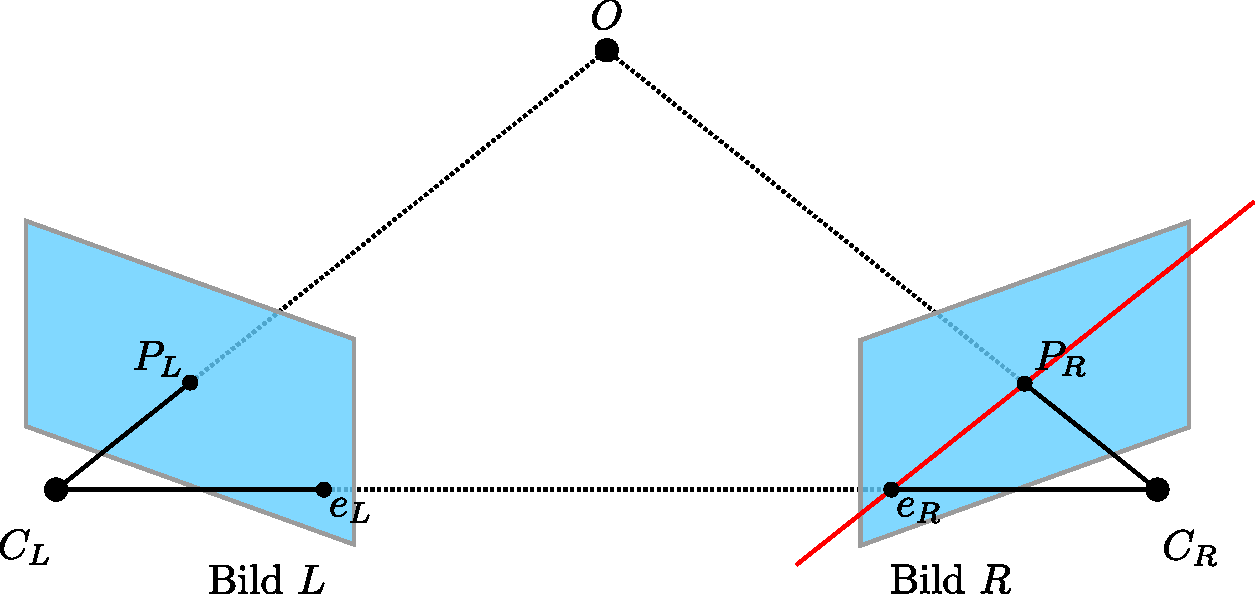
\includegraphics[width=10cm]{img/epipolar_geometry.pdf}
	\end{center}
	\caption{Darstellung der Epipolargeometrie.}
	\label{fig:epipolar_geometry}
\end{figure}

\noindent
Abbildung \ref{fig:epipolar_geometry} visualisiert diesen Prozess. Gegeben sind die beiden Projektionszentren $C_L$ und $C_R$ der beiden Bildebenen, welche im Zuge der Kalibrierung mitbestimmt werden, sowie die Bildpunkte $P_L$ und $P_R$, welche beide die Position des Objektpunktes $O$ in beiden Bilden beschreiben. Zunächst ist es nur möglich den Strahl auf dem sich $O$ befindet zu bestimmen.Aufgrund des Wissens der relativen Orientierung der Kameras können mithilfe der Basislinie zwischen den beiden Kameras die Epipole in $L$ und $R$ ermittelt werden. Rechnerisch ergibt sich die Epipolarlinie aus der Multiplikation des Bildpunktes mit der Fundamentalmarix. Betrachtet man den Strahl $C_L,O$ aus Perspektive des rechten Bildes, und verschiebt $O$ entlang dessen, so ergibt sich die Epipolarlinie in $R$.Somit ist es möglich mithilfe der vorhandenen Epipole $e_L$, $e_R$ die Epipolarlinie $e_l,P_{x_2,y_2}$ zu bestimmten. Anhand dieser kann der Suchraum für den gesuchten korrespondierenden Bildpunkt im Rechten Bild auf die Epipolarlinie eingegrenzt werden. Kann der Punkt mittels eines \emph{Matching}-Ansatzes gefunden werden, ist es möglich die 3D Position des Objektpunkts zu triangulieren.\\
\noindent
Generell sind die Epipole durch den Schnittpunkt der Basislinie mit den beiden Bildebenen definiert. Im Falle eines Stereonormalfalles jedoch ist ein Schnittpunkt der Basislinie mit den Bildebenen nicht möglich, sodass die Epipole in der Unendlichkeit und parallel zur x-Achse liegen. Dies hat unter anderem den Vorteil, das die Epipolargeometrie bereits bekannt ist, und korrespondierende Bildpunkte nur noch innerhalb einer Pixelreihe gesucht werden müssen.


\section{Kamerakalibrierung und Rektifizierung}
\label{sec:camera_calibration}
Um den Prozess der Korrespondenzanalyse zu vereinfachen und beschleunigen bietet die Rektifizierung der Referenzbilder einen simplen Einstiegspunkt zur Lösung des Stereo-Korrespondenzproblems. Dafür müssen zunächst die intrinsischen und extrinsischen Parameter der Kamera berechnet werden. Die Ermittlung der intrinischen Parameter ist dabei der Hauptbestandteil der Kalibrierung. Mit Hilfe weitere Schritte kann auch die relative Orientierung ermittelt werden. Zu Beginn des Kalibrier-Prozesses werden Bilder eines Kalibrierobjektes aufgenommen. Dies ist meistens ein einfaches Schachbrettmuster mit ungleicher Anzahl an Quadraten, oder auch ein radiales Objekte mit einem spezifischerem Aufbau. Die Dimensionen des Kalibrierobjektes sind dabei bekannt. Der Prozess der Kalibierung zielt darauf ab die \enquote{inneren} Parameter der Kamera zu bestimmen. Dies beinhaltet einerseits die Kameramatrix in welcher Parameter wie der Fokus Punkt(Focal Point), der Bildhauptpunkt(Principal Point) sowie die Brennweite der der Kamera. Weiterhin werden geometrische Verzerrungen des Bildes, beispielsweise Radiale Verzeichnungen durch die verwendete Optik, parametrisiert und somit nutzbar für die Entzerrung der Bilder in weiteren Schritten. Weiterhin werden bei der Kalibrierung die extrinsischen (äußeren) Parameter, d.h. die relative Orientierung der beiden Kameras zueinander, bestimmt. Zu diesen zählt die Translation (x, y und z) sowie die Rotation der Kamera um die jeweiligen Achsen des Weltkoordinatensystems (ausgedrückt durch drei Winkel). Ein spezieller Aspekt bei der Kalibierung von Stereo-Systemen ist die Berechnung der extrinsischen Parameter von einer Kamera zur anderen. Die dabei berechnete Translation einer Kamera zur Referenzkamera wird als Basislinie bezeichnet. Die Kenntnis über die relative Orientierung von Stereo-Kameras führt dazu, dass man identifizierte korrespondierende Punkte in den Bildpaaren direkt metrisch triangulieren kann. Der Prozess der Parameterfindung ist in der Regel ein Prozess welcher einmalig nach dem Aufbau ausgeführt werden muss und solange währt, wie sich nichts am Aufbau der Kameras ändert (Optik, Translation, Rotation).\\

\noindent
Folgend aus der Kalibrierung der Kameras beginnt der Prozess der Rektifizierung der Bilder. Dieser kann dabei in zwei Schritte unterteilt werden, zunächst die Rektifizierung der Bilder, anschliessend die Berechnung der ROI. Mithilfe der zuvor berechneten intrinsischen und extrinsischen Parameter kann nun die Transformation der beiden Kamerabilder zueinander berechnet werden. Dabei werden die durch die Kalibrierung erhaltenen Objektpunkte unter dem Aspekt der Epipolargeometrie paarweise rotiert, sodass die Epipole beider Bilder auf der x-Achse liegen. Nach Verschiebung der Epipole entlang der X-Achse ins Unendliche ist Parallelität der Epipolarlinien gewährleistet. Daraus resultieren parallele und orthogonale Blickrichtungen zur identischen Bildebene, somit sind beide Bildebenen Element derselben Ebene. Die finale ROI ergibt sich aus der Konjuktion der einzelnen ROI's. Nach der Rektifizierung und dem Anwenden der ROIs auf beiden Kamerabildern entspricht die jeweilige Pixelreihe im linken Bild der Pixelreihe mit dem selben Index im rechten Bild. Abbildung \ref{img:rectification} verdeutlicht den Ablauf der Rektifizierung, so ist in Abbildung \ref{img:rectification} (c) erkennbar das sich die korrespondierenden Bildpunkte auf einer Epipolarlinie befinden.\\

\begin{figure}[h]
	\centering
	\begin{tabular}{c}
	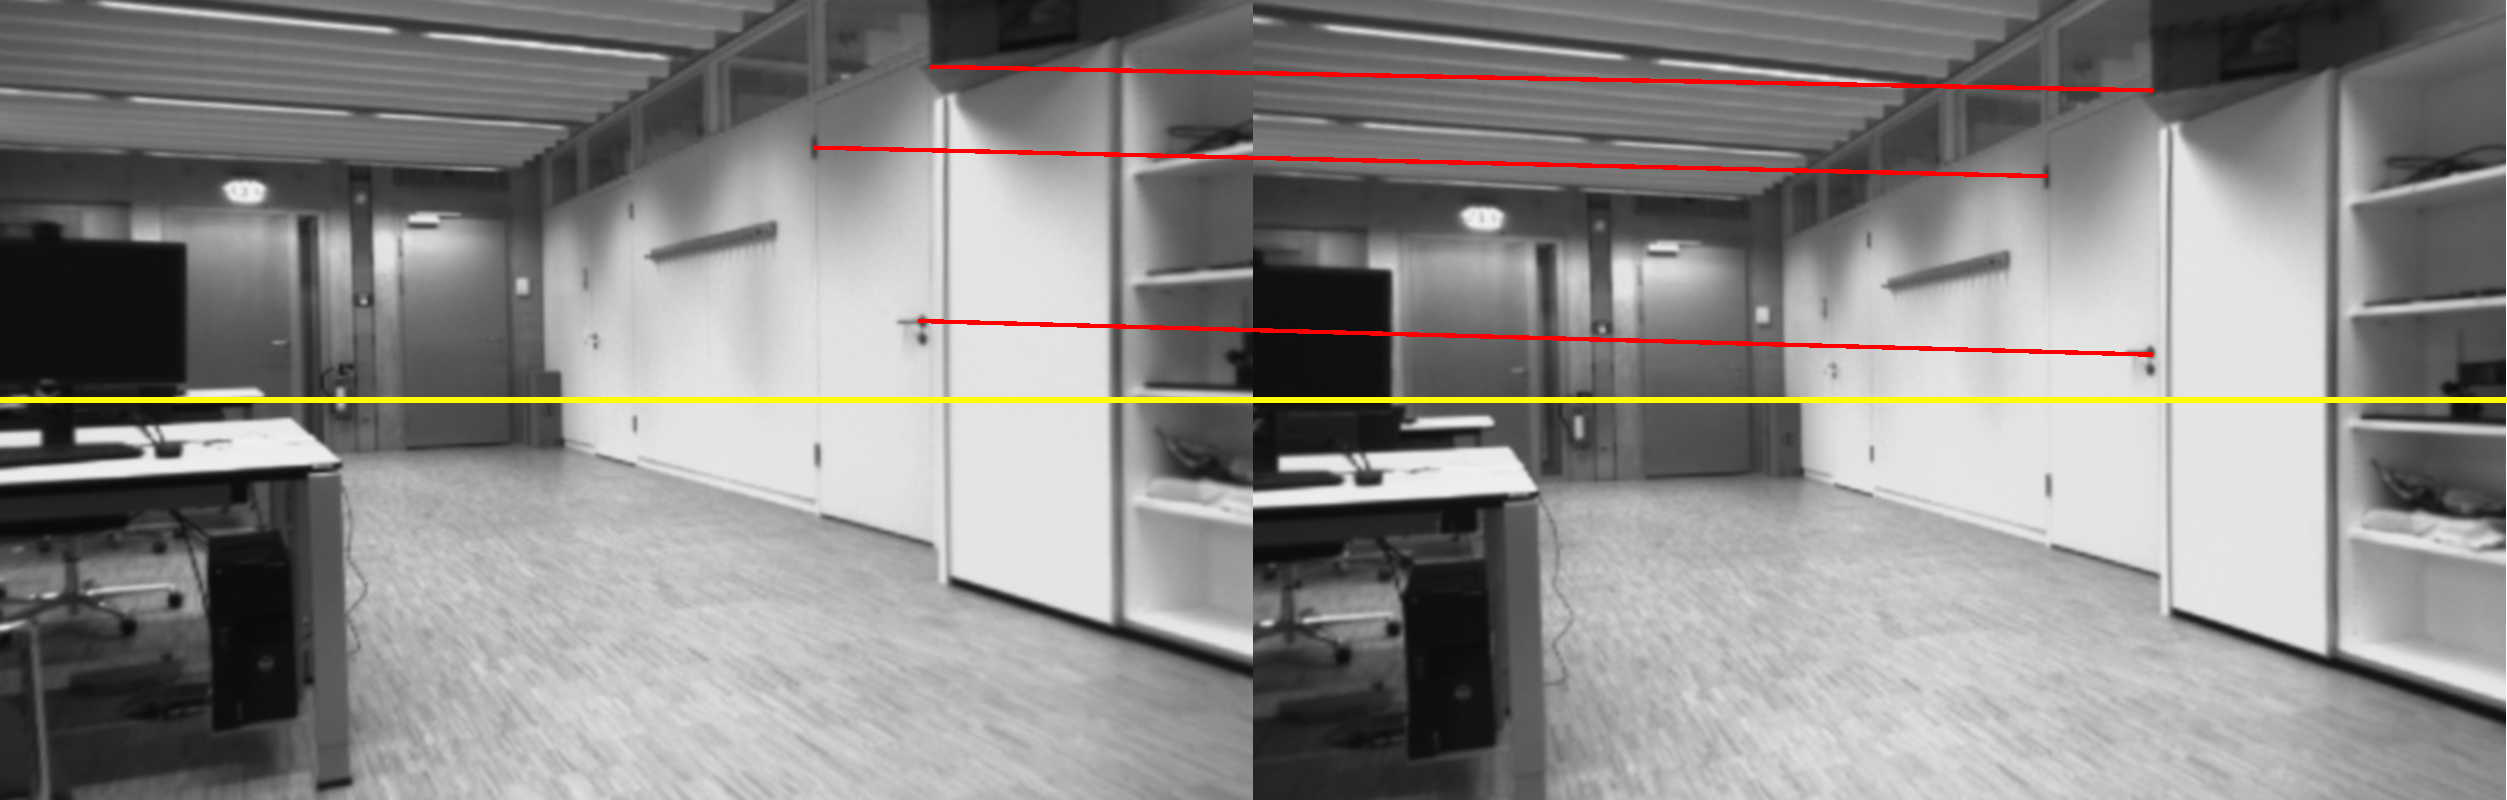
\includegraphics[width=10cm]{img/calibration/undistort}\\
	\small (a) Korrespondierende Punkte innerhalb der entzerrten Bilder.\\\\
	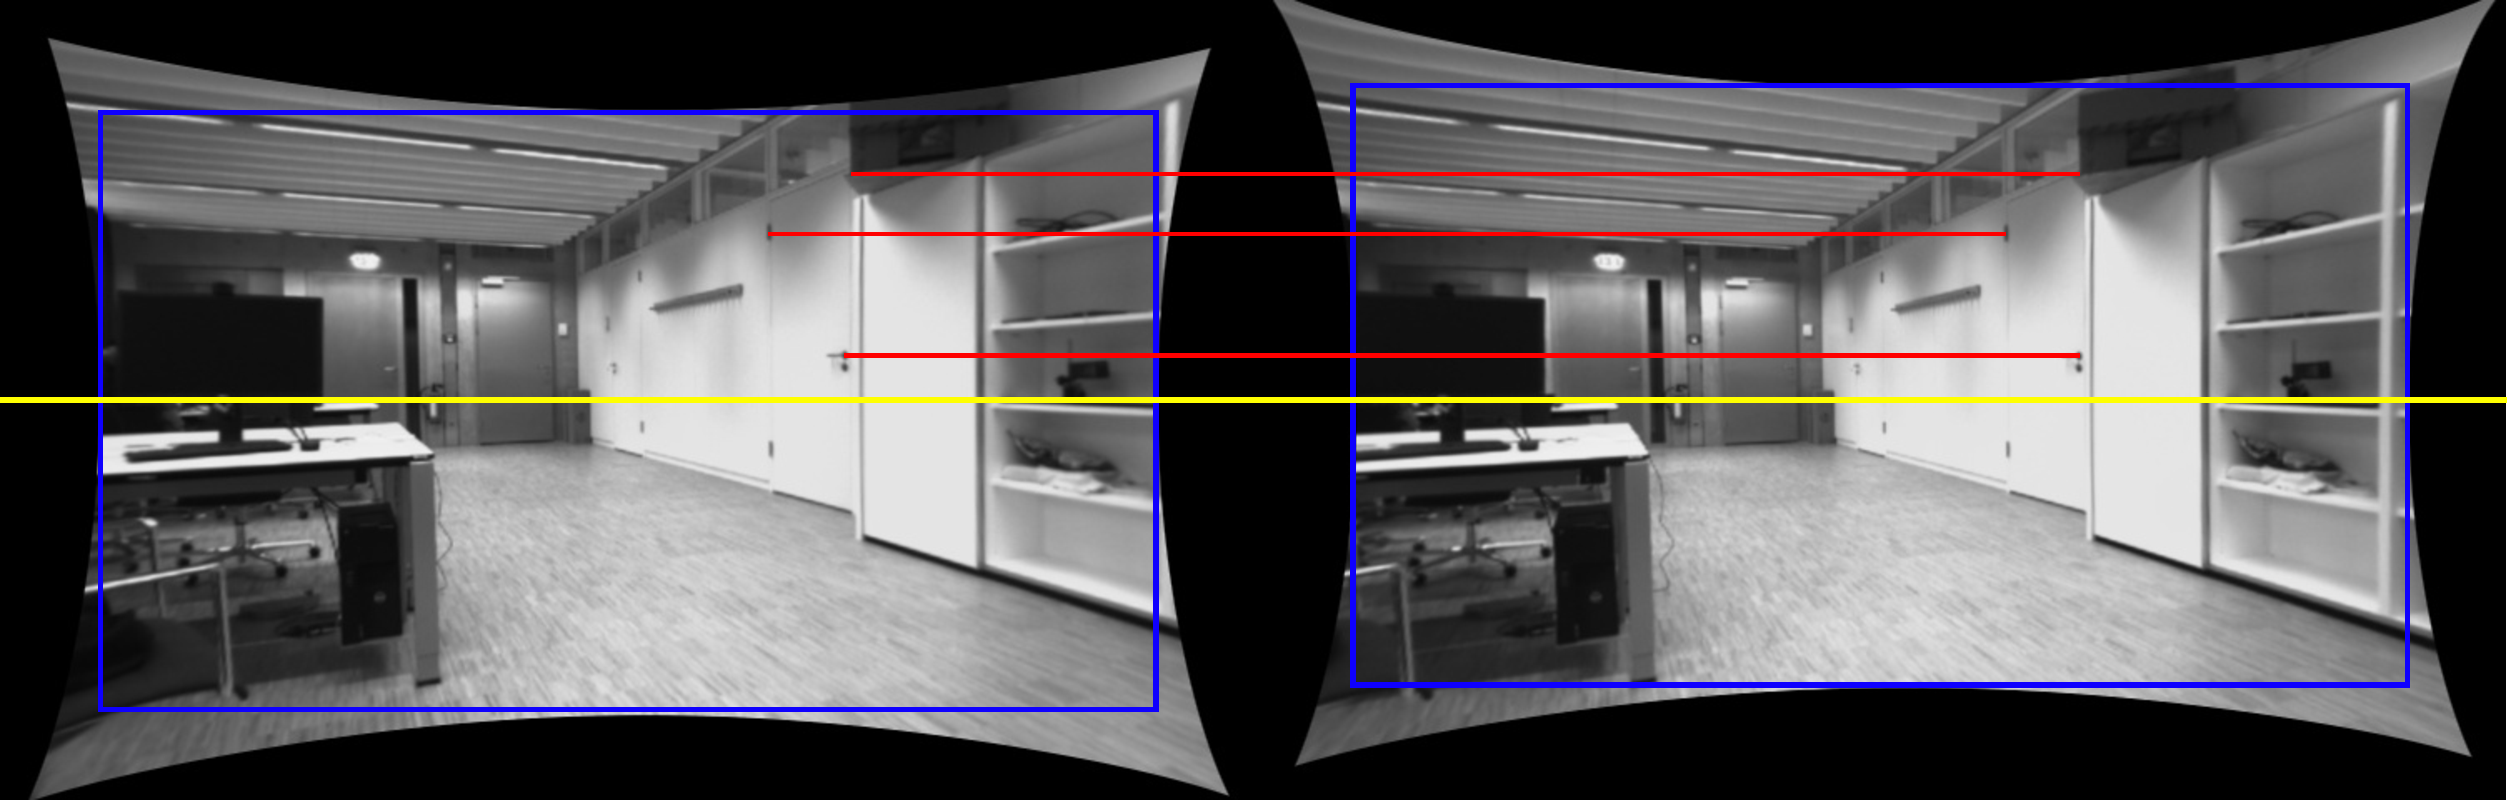
\includegraphics[width=10cm]{img/calibration/rect_uncropped.pdf}\\
	\small (b) Korrespondierende Punkte in den rektifizierten Bildern. \\Die ROIs (blau) kennzeichnen die jeweils maximal \\möglichen rechteckigen Flächen.\\\\
	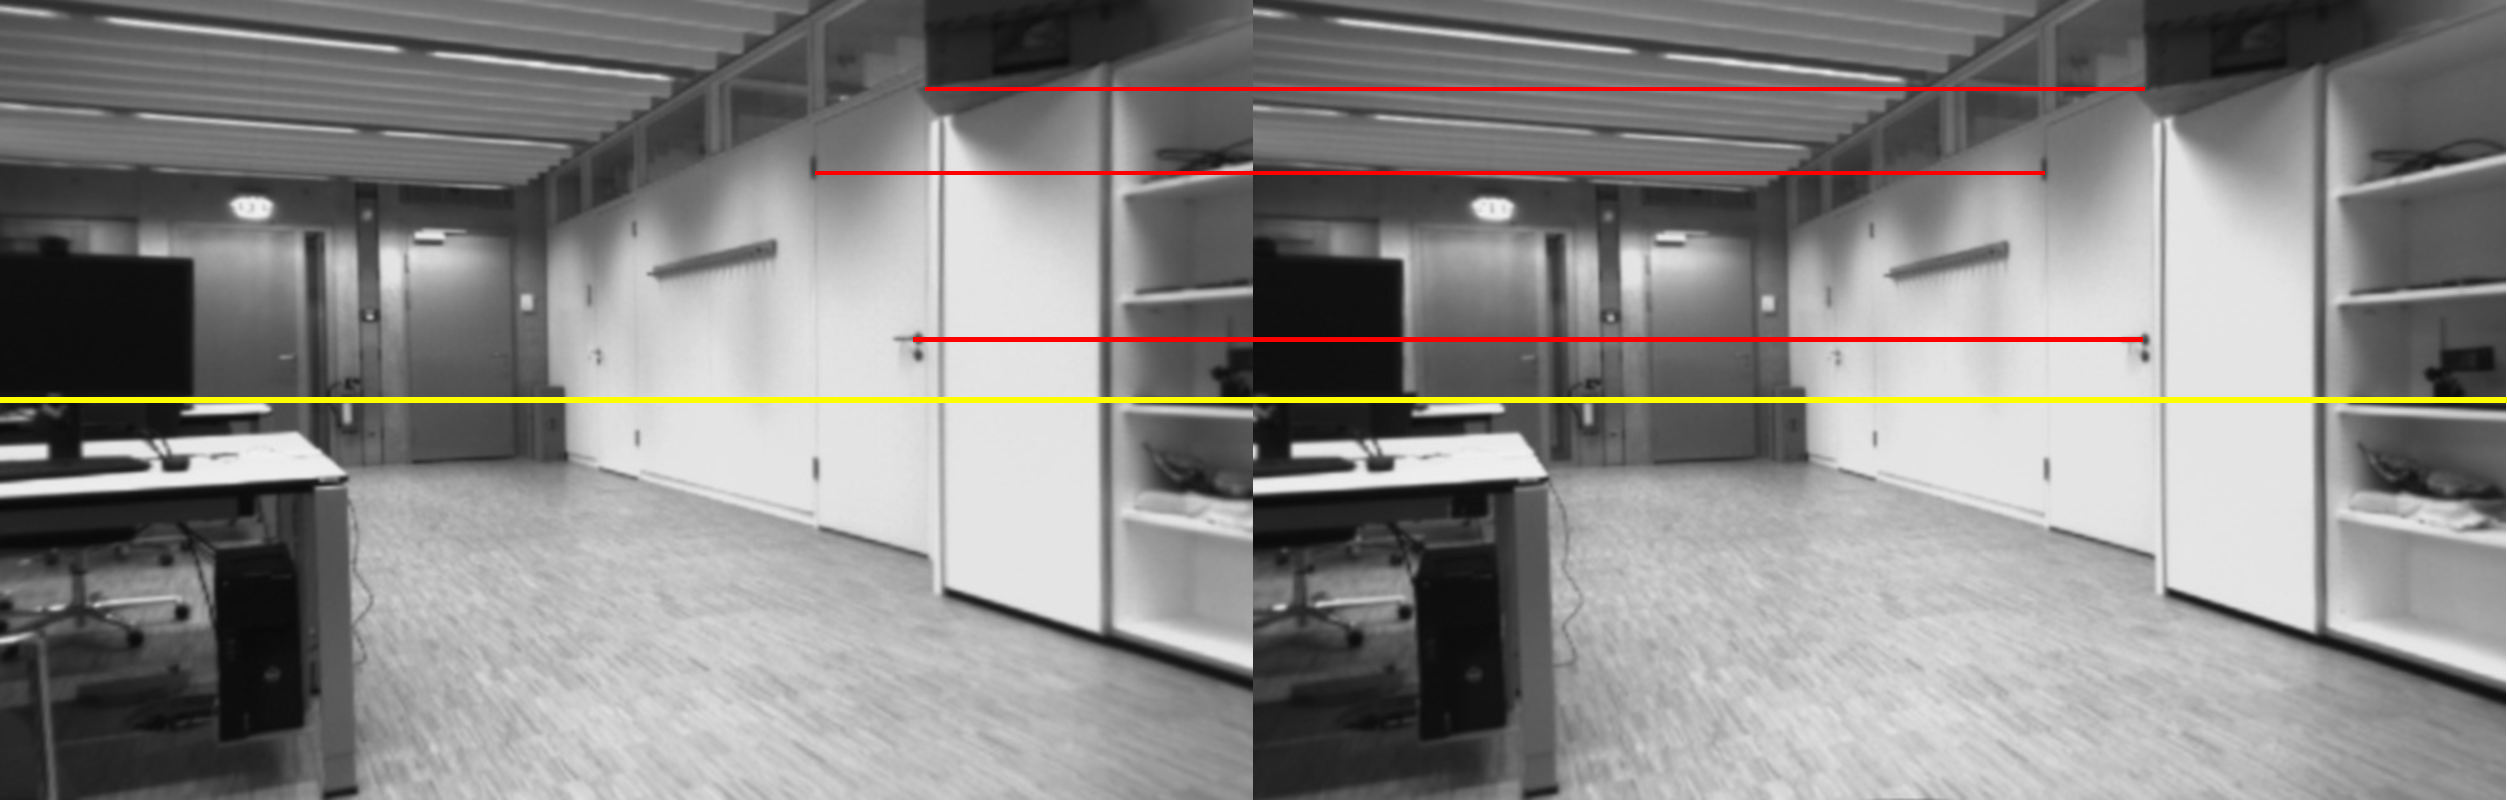
\includegraphics[width=10cm]{img/calibration/rect_cropped.pdf}\\
	\small (c) Korrespondierende Punkte in den beschnittenen, skalierten\\ und rektifizierten Bildern. \\
	\end{tabular}
\caption{Ablauf der Rektifizierung}
\label{img:rectification}
\end{figure}

% ---------------------- section -----------------------
\section{Stereo Matching}
\label{sec:stereo_matching}
Das grundlegende Konzept des \emph{Stereo Matchings} beschreibt das Finden korrespondierender Punkte in zwei Bildern. Die Position der beiden Kameras ist dabei leicht versetzt, um einen jeweils anderen Blickwinkel auf die Szene zu erhalten. Mithilfe der verschiedenen Perspektiven können Disparitäten zwischen korrespondierenden Pixeln berechnet werden. Die räumlichen 3D-Koorinaten der aufgenommenen Szene stehen im direkten (funktionalen) Zusammenhang mit der Information über Disparität, der  relativen Orientierung der Kameras sowie der Kamerakalibrierung. Durch die Transformation zum Stereonormalfall vereinfacht sich dieser Zusammenhang enorm. Im Laufe dieses Prozesses kommt es zu zwei wesentlichen Problemstellungen: die Berechnung der Disparität (Stereo Korrespondenz) sowie die Invertierung der projektiven Geometrie, um dreidimensionale Informationen aus der errechnetet Disparität zu erhalten. Sofern eine Lösung beider Probleme vorhanden ist, können diese Informationen durch einfache Triangulierung errechnet werden.

\subsection{Lokale Methoden}
\label{subsec:local_methods}
Zur Berechnung der Disparität in lokalen \emph{Stereo Matching} Algorithmen gilt grundlegendes Prinzip: “Finde Pixel $P_2$ korrespondierend zu $P_1$ im Referenzbild”. Dabei wird die Korrelation von $P_1$ und $P_2$ unter Einbezug der lokalen Nachbarschaft bestimmt und die maximale Korrelation als Indikator für die Übereinstimmung von Pixeln herangezogen. Der Referenzpunkt ist dabei das Zentrum eines Bereiches in welchem das Matching ausgeführt wird. Geläufige Methoden dafür sind \emph{Sum of Absolute Differences} (SAD) (Hirschmüller 2011), \emph{Zero-mean Normalized Cross-Correlation} (ZNCC) (Chen \& Medioni, 1999), (Sára, 2002), \emph{Sum of Squared Differences} (SSD) (Cox et al., 1996). Jedoch können aufgrund des recht einfachen Ansatzes, der bei starken perspektivischen Änderungen und untexturierten Bereichen keine sinnvollen Ergebnisse liefert, falsche Berechnungen der räumlichen Tiefe auftreten, da benachbarte Pixel verschiedene Disparitäten aufweisen können (beispielsweise an horizontalen Kanten wie Türrahmen etc.). Strukturell gesehen sind lokale Methoden einfacher gehalten als globale Methoden, wodurch ein hoher Grad an Optimierung in der Implementierung möglich ist.

\subsection{Globale Methoden:}
\label{subsec:global_methods}
Bei globalen \emph{Stereo Matching} Algorithmen wird ein globales Modell der zu betrachtenden Szene erstellt sowie eine ebenfalls globale Kostenfunktion definiert, welche es zu minimieren gilt. Dabei werden im Gegensatz zu lokalen Methoden die Korrespondenzen in einer Pixelreihe und die des gesamten Bildes miteinander verglichen. Zur Vereinfachung dieses Vorgangs betrachten einige Algorithmen nur die durch die Epipolargeometrie vorgegebenen Bildbereiche, wodurch ein zweidimensionales Problem auf ein eindimensionales reduziert wird. Resultierend daraus liegt die Stärke globaler Methoden in der Bewältigung schwacher Texturen sowie auftretender Okklusionen und unterschiedlicher Lichteinfälle, was, aufgrund der höheren Komplexität in einem höheren Rechen- und Speicheraufwand mündet. Weitere Verbesserungen der Ergebnisse können durch Techniken wie Dynamische Programmierung und Graph Cut erreicht werden.
% TODO JENS referenzen gibt es in meinen quellen zu lokalen und globalen --> buecher

\subsection{Block Matching}
\label{subsec:stereo_matching_bm}
Einen der einfachsten Ansätze zur Berechnung von Korrespondenz zwischen zwei Bildern bietet der Block Matching Algorithmus. Bei dieser lokalen Methode werden Blöcke bestimmter Größe mithilfe von Korrelation(Vergleich zweier Signale auf Übereinstimmung) auf Korrespondenz untersucht. Dabei reduziert die Epipolargeometrie diesen Prozess auf ein eindimensionales Problem, so dass ein Block im linken Bild mit allen potentiell möglichen Blöcken auf der Epipolarlinie des rechten Bildes vergleichen wird. Das eigentliche Matching erfolgt über die Berechnung des gewählten Korrelationswerts eines Blockes mithilfe einer Energiefunktion.

\begin{figure}[h]
	\begin{center}
		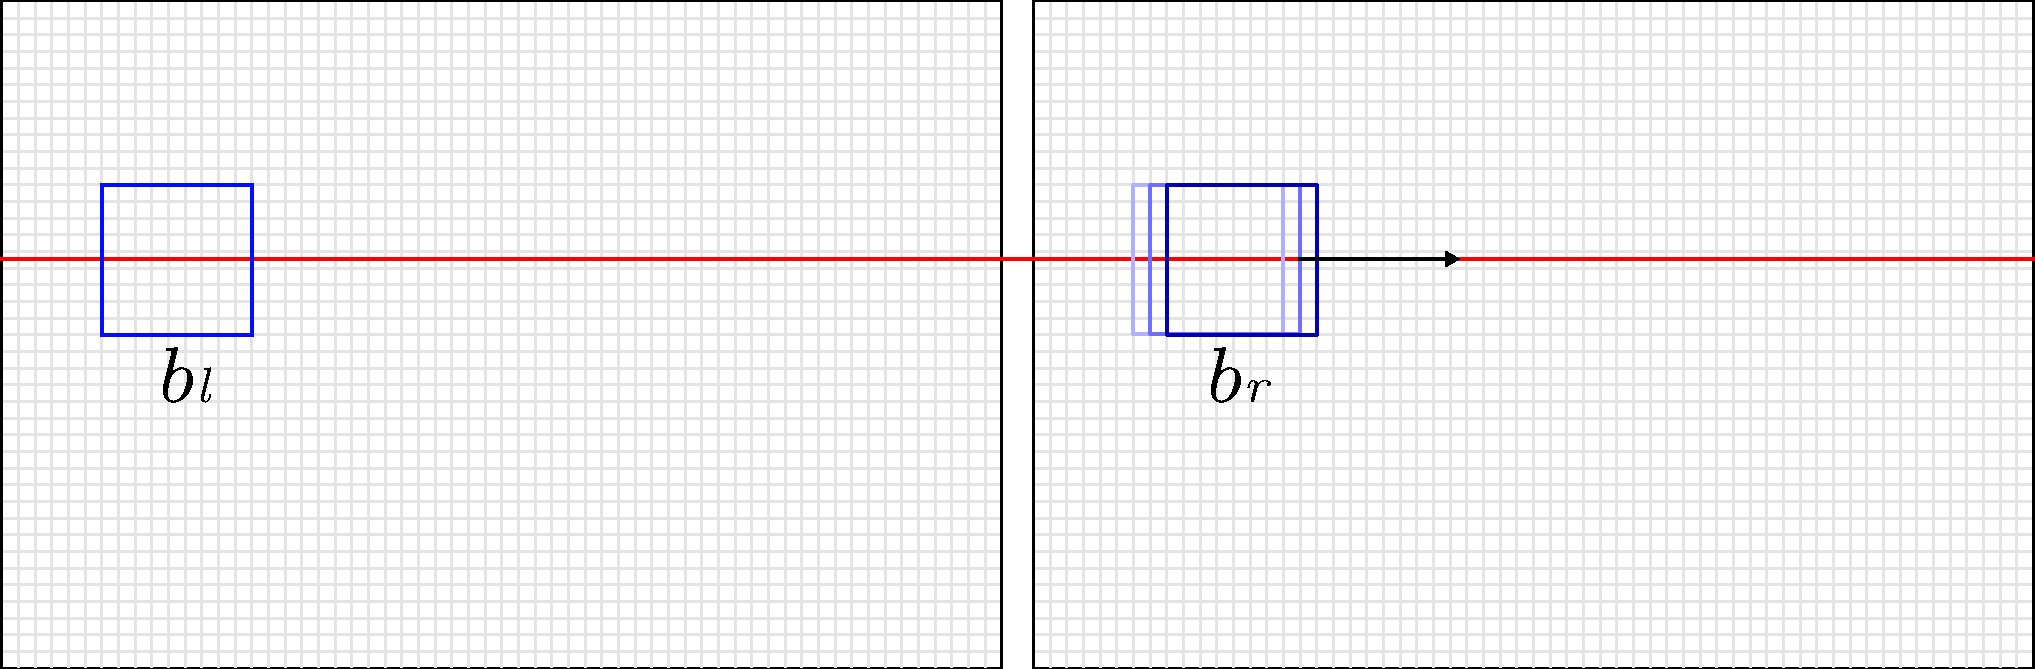
\includegraphics[width=10cm]{img/block_matching.pdf}
	\end{center}
	\caption{Visualisierung des Block Matching Algorithmus}
	\label{fig:block_matching}
\end{figure}

\noindent
Diesen Prozess veranschaulicht Abbildung \ref{fig:block_matching} . Durch den Fokus auf einzelne Pixelreihen und deren unmittelbare Umgebung ist dieses Verfahren wesentlich schneller, aber auch ungenauer als globale Matching Algorithmen. 
 

\subsection{Semi Global Block Matching}
\label{subsec:stereo_matching_sgbm}
Das im Rahmen dieser Arbeit verwendete Verfahren zur Berechnung von Disparity Maps ist der in der freien Computer Vision Bibliothek OpenCV \cite{opencv} implementierte \emph{Semi Global Block Matching} Algorithmus. Diese leicht abgewandelte Implementierung des \emph{Semi Global Matching} (SGM) Algorithmus von Hirschmüller et. al \cite{hirschmuller2005sgm} zeichnet sich sowohl durch seine Genauigkeit, als auch durch seine performante Berechnung aus. Unter Zuhilfenahme dieses Verfahren ist es möglich, Disparitätenkarten in Echtzeit zu berechnen. Im Folgenden wird zunächst die grundlegende Funktionsweise des SGM erläutert. Im Anschluss daran werden die Unterschiede zum SGBM herausgearbeitet sowie eine kurze Erklärung der Parameter dessen vorgenommen.\\

\noindent
\textbf{SGM:} \\
Die grundlegende Idee des Semi-Global Matching Algorithmus besteht in dem pixelweisen Matching von Mutual Information \footnote{\emph{Mutual Information}(MI), zu deutsch Transinformationen, beschreiben den statistischen Zusammenhang zweier Zufallsgrößen. Genauer gesagt beschreiben sie die Höhe des Informationsgehaltes einer Zufallsvariable aus anderen zufällig gewählten Werten.}. Ausgangsvorraussetzung dafür sind verschiedene Bilder derselben Szene mit vorhandener und bekannter Epipolargeometrie. Ein weiteres Kernelement des SGM ist die Anwendung eines globalen zweidimensionalen Glattheitskriteriums, was durch die Kombination mehrerer eindimensionaler Beschränkungen approximiert wird. Zunächst werden für jeden Pixel $P$ aus der Intensität $I_{bp}$ sowie der vermuteten Korrespondenz $I_{mq}$ auf der Epipolarlinie $q=e_{bm}(pd)$ die Matching Kosten berechnet. Zur Berechnung der MI wird zunächst eine initiale Disparitätenkarte benötigt. Diese wird nach dem Ansatz von Kim et al \cite{lee2012intelligent} zufällig gewählt, um die Kosten berechnen zu können. Zur Steigerung der Performanz wird die Disparitätenkarte zunähst nur auf halber Auflösung berechnet, wodurch der Rechenaufwand um den Faktor $8$ reduziert wird. Zur Vermeidung falscher Kostenberechnungen durch auftretendes Rauschen innerhalb des Bildes werden benachbarte Disparitäten mit in die Berechnungen einbezogen.\\

\noindent
Das letzte Problem besteht in der Berechnung der Korrespondenz sowie der daraus resultierenden Disparitäten. Dabei wird nach der Disparität $D$ mit der geringsten berechneten Energiefunktion gesucht. Anstatt nun einfach den minimalsten Pfad der Kosten zu summieren, werden zusätzlich auch andere Richtungen zur aktuellen Disparität mit einbezogen (siehe Abbildung \ref{fig:sgm_directions}).

\begin{figure}[h]
	\centering
	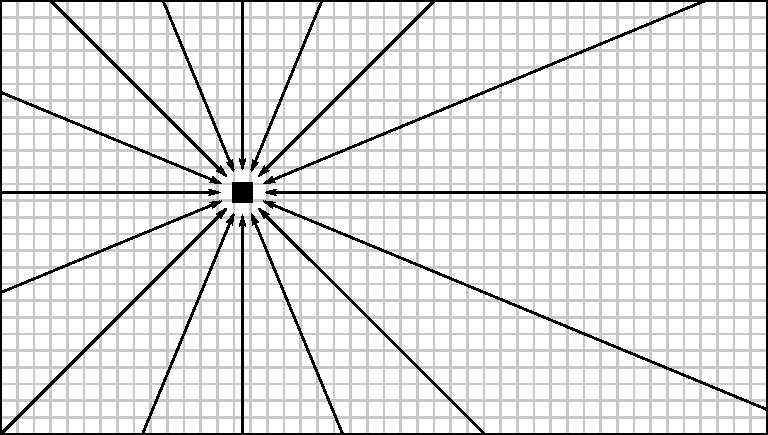
\includegraphics[width=8cm]{img/sgm_directions.pdf}
	\caption{Darstellung der verschiedenen Richtungen}
	\label{fig:sgm_directions}
\end{figure}

\noindent
Zur Berechnung valider Werte sollten dabei mindestens 8 Richtungen vorliegen, eine vermehrte Anzahl an Richtungen, etwa 16, ist dabei vorteilhaft. Die berechnete Disparität ergibt sich aus den minimalen Kosten anhand dieser Pfade.\\

\noindent
\textbf{SGBM:} \\
Der \emph{Semi Global Block Matching} Algorithmus ist ein in der Computer Vision Library OpenCV implementiertes Verfahren zur schnellen Berechnung von Disparitätenkarten. Die Grundlage dafür bietet Hirschmüller et al.’s SGM \cite{hirschmueller2008sgm} mit den folgenden grundlegenden Änderungen:

\begin{enumerate}[label=C.\arabic*]
	\item Statt den originalen 8 bzw. 16 Richtungen werden nur 5 betrachtet. \label{item:differences_directions}
	\item Es werden  standartm\"assig keine einzelnen Pixel sondern Blöcke verglichen. \label{item:differences_matching}
	\item Anstelle der Mutual Information Kostenfunktion wird das von Birchfield et al. vorgestellte Sub-Pixel \emph{Dissimilarity Measurement} Verfahren verwendet \cite{birchfield-tomasi}.
	\item Verschiedene Schritte der Vor- und Nachprozessierung des \emph{StereoBM} Algorithmus werden verwendet, dazu zählen Filtermethoden wie quatdratische Interpolation oder Sprenkelfilter.
\end{enumerate}

\noindent
Dies ermöglicht eine schnelle Berechnung der Disparitäten auf einem qualitativ hochwertigen Niveau. Der geringe Verlust an Qualität, hervorgerufen durch die geringere Anzahl an betrachteten Richtungen, kann in Anbetracht der Berechnung in Echtzeit vernachlässigt werden.

\begin{figure}[h]
\centering
	\begin{tabular}{m{2cm} m{3.3cm} m{3.3cm} m{3.3cm}}
	{\scriptsize Datensatz}&
	\begin{center} {\scriptsize Tskukuba} \end{center} &
	\begin{center} {\scriptsize Teddy} \end{center} &
	\begin{center} {\scriptsize Cones} \end{center}
	\\
	{\scriptsize Bilder links} &
	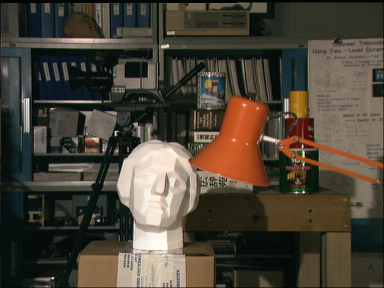
\includegraphics[width=3cm]{img/disparity_images/left_tsukuba.png} & 
	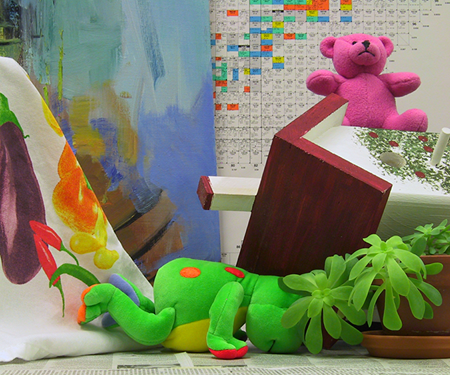
\includegraphics[width=3cm]{img/disparity_images/left_teddy.png} & 
	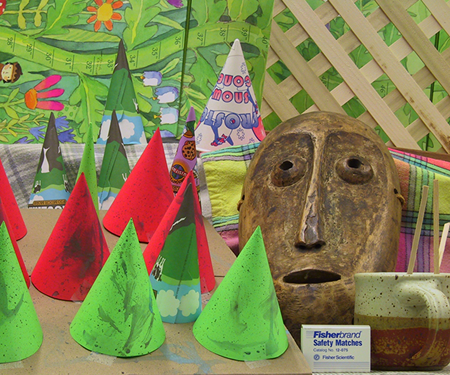
\includegraphics[width=3cm]{img/disparity_images/left_cones.png} 
	\\ 
	{\scriptsize Ground Truth} &
	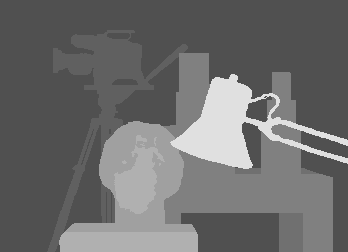
\includegraphics[width=3cm]{img/disparity_images/gt_tsukuba.png} & 
	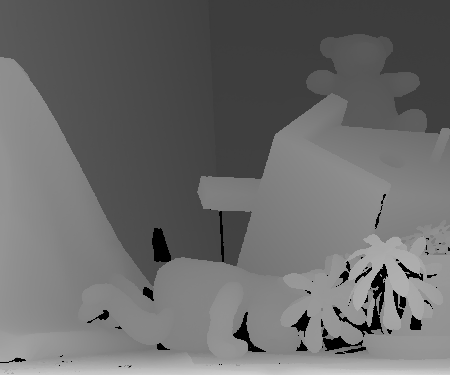
\includegraphics[width=3cm]{img/disparity_images/gt_teddy.png} & 
	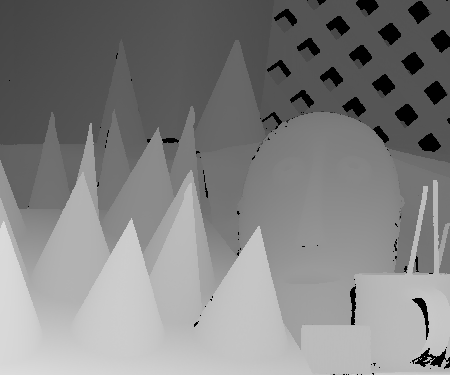
\includegraphics[width=3cm]{img/disparity_images/gt_cones.png} 
	\\
	{\scriptsize SGM (MI)} &
	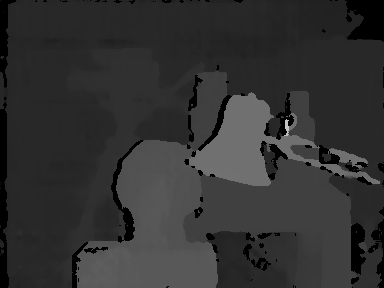
\includegraphics[width=3cm]{img/disparity_images/sgm_tsukuba.png} &
	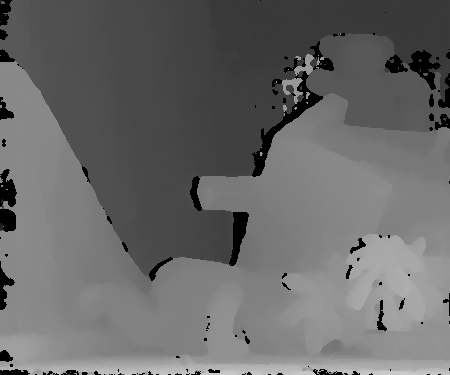
\includegraphics[width=3cm]{img/disparity_images/sgm_teddy.png} &
	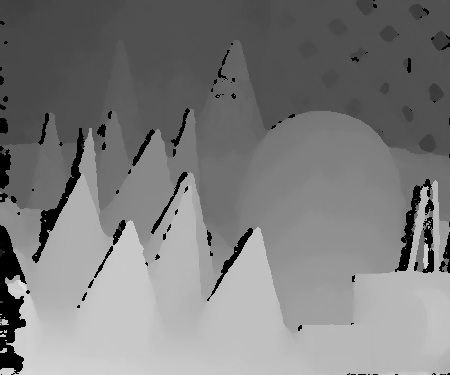
\includegraphics[width=3cm]{img/disparity_images/sgm_cones.png}
	\\ 
	{\scriptsize SGBM} &
	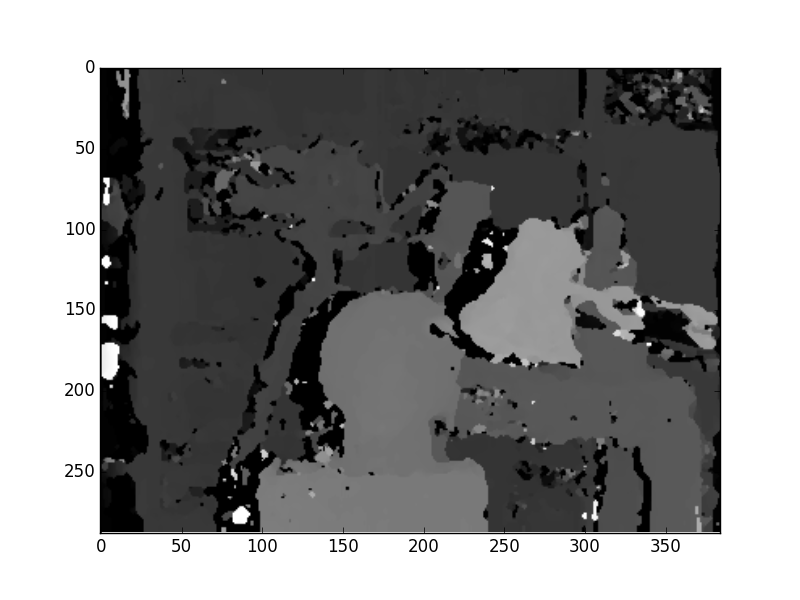
\includegraphics[width=3cm]{img/disparity_images/sgbm_tsukuba.png} &
	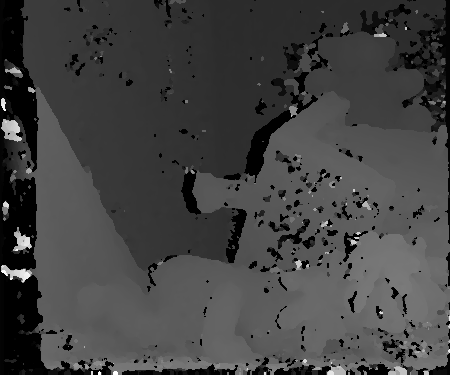
\includegraphics[width=3cm]{img/disparity_images/sgbm_teddy.png} &
	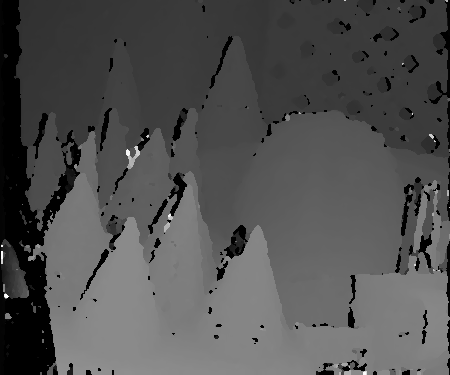
\includegraphics[width=3cm]{img/disparity_images/sgbm_cones.png}
	 \\ 
	\end{tabular}
\caption{Vergleich zwischen Ground Truth Bildern sowie dem SGM(2005) und OpenCV's SGBM}
\label{fig:disparity_comparison}
\end{figure}
% TODO vielleicht eigene Bilder verbessern, sodass tsukuba nicht ganz so crappy aussieht

\noindent
Abbildung \ref{fig:disparity_comparison} stellt die originalen Bildern der Szene (\cite{middlebury_data}), die mithilfe von strukturiertem Licht aufgenommenen Ground Truth Bilder sowie die jeweiligen berechneten Tiefenkarten durch den SGM und den SGBM dar. Aus dieser ist der Qualitätsverlust des SGBM beim Tsukuba- sowie beim Teddy Datensatz zu erkennen. Trotz dessen sind die Grundformen sowie die berechnete Tiefe klar erkennbar. Grundlegend bietet der SGBM eine sowohl qualitativ hochwertige Berechnung von Tiefenkarten. Kleinere qualitative Einbußen, durch das Matching einzelner Blöcke anstelle von Pixeln können daher bei steigender Performance akzeptiert werden.\\

\noindent\
Weiterhin existiert eine Reihe verschiedener Parameter welche die Berechnung der Disparity Map aktiv beeinflussen. Im folgenden werden die zur Initialisierung obligatorischen Parameter in ihrer Funktionsweise grob beschrieben.

\begin{itemize}
	\item \textbf{\emph{minDisparity:}}\\
	Der Parameter \emph{minDisparity} begrenzt den messbaren Tiefenbereich nach oben, dies ist vor allem dann von Nöten wenn die Tiefenberechnung nach unten hin abgegrenzt werden soll. Er beschreibt also die minimale zu erkennende Disparität
 	\item \textbf{\emph{numDisparities:}}\\
 	Mit Hilfe der Number of Disparities \emph{numDisparities} wird die Breite des Matchingbereiches festgelegt. Er definiert wie viele Pixel im linken Bild auf Korrespondenz im rechten Bild analysiert werden sollen. In Abhängigkeit der Größe des Parameters entsteht bei der Berechnung der Tiefenkarte ein Bereich in welchem keine Informationen enthalten sind. Die damit verbundene weitere Verfahrensweise wird im Abschnitt \ref{sec:preprocessing} \enquote{Preprocessing} näher erläutert.
	\item \textbf{\emph{blockSize:}}\\
	Die \emph{blockSize} des \emph{SGBM} beschreibt die Größe des Matching Blocks in Pixeln. Je größer der Wert gewählt wird, desto weicher wird die resultierende Disparity Map. Dabei gehen jedoch auch Informationen verloren. Ist der Wert niedrig so ist es unter Umständen schwerer homogene Flächen korrekt zu Matchen und es treten mehr nicht-korrespondierende Bereiche auf.
\end{itemize}

% ---------------------- section -----------------------
\section{mvStereoVision Framework}
\label{sec:framework}
Das verwendete Framework zur Bildaufnahme und Disparity Map Berechnung wurde bedient sich der von Matrix Vision zur Verfügung gestellte Bibliothek \cite{matrixvision} zur Kommunikation mit den Kameras, sowie OpenCV \cite{opencv} zur Verarbeitung der Bilder. Die wesentlichen Funktionen werden im folgenden näher beleuchtet.\\

\noindent
\textbf{Bildaufnahme:}\\
Die Aufnahme der einzelnen Bilder beginnt bei einer Anfrage an die Kamera nach den jeweiligen Rohdaten. Diese werden anschliessend mithilfe der durch die Kalibrierung ermittelten Parameter entzerrt und rektifiziert und liegen so zur weiteren Verarbeitung bereit. Die Aufnahme der Bilder erfolgt dabei in separaten Threads um unabhängig von weiteren Berechnungen Bilder aufzunehmen. Die Berechnung der Disparity Map erfolg ebenfalls in einem eigenen Thread. Sofern eine neue Disparity Map vorliegt wird innerhalb des Hauptprogramms mit Hilfe eines Wahrheitswertes darüber informiert das diese vorliegt. Der gesamte Prozess wird in Abbildung \ref{fig:framework_pipeline} visualisiert.\\

\begin{figure}[h]
	\begin{center}
		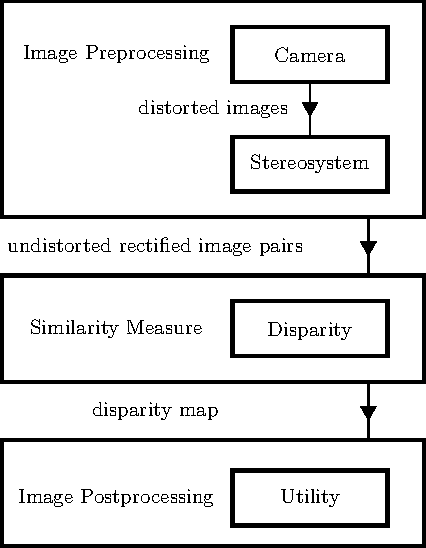
\includegraphics[width=6cm]{img/framework_pipeline.pdf}
	\end{center}
	\caption{Ablauf der Bildaufnahme, Disparity Map Berechnung sowie weiteren Verarbeitung}
	\label{fig:framework_pipeline}
\end{figure}


\noindent
\textbf{Distanzberechnung:}\\
Zugrundeliegend bei der Distanzberechnung ist die Reprojektionsmatrix $Q$ welche im Rahmen der Rektifizierung berechnet wird und wie folgt aufgebaut ist.
\begin{equation}
    Q= 
    \begin{bmatrix}
      1 & 0 & 0 & -C_x\\
      0 & 1 & 0 & -C_y\\
      0 & 0 & 0 & f\\
      0 & 0 & \frac{-1}{T_x} & \frac{C_x - C_x'}{T_x}
    \end{bmatrix}
    \longrightarrow
    \begin{bmatrix}
      1 & 0 & 0 & -C_x\\
      0 & 1 & 0 & -C_y\\
      0 & 0 & 0 & f\\
      0 & 0 & a & b
    \end{bmatrix}
\end{equation}
Dabei beschreiben $-C_x$ und $-C_y$ die beiden negativen Koordinaten des Bildhauptpunktes der Referenzkamera, beispielsweise der linken. Der Parameter $f$ die Brennweite der linken Kamera. $T_x$ ist die horizontale Translation zwischen beiden Kameras. Die in der Q-Matrix enthaltenen Parameter sind mit Ausnahme von $C_x'$ alle die der linken Kamera. Es wird angenommen das sich die beiden Strahlen der Bildhauptpunkte in der Unendlichkeit schneiden. Dies führt zu einer Annäherung des unteren rechten Parameters an $0$. Zur Einfacheren Darstellung und Erläuterung werden die Basislinie der Kamera $\frac{-1}{T_x}$ im folgenden als $a$ sowie die Darstellung beider Bildhauptpunkte $\frac{C_x - C_x'}{T_x}$ als $b$ notiert.\\

\noindent
Eine Eigenschaft der Reprojektionsmatrix ist die einfache Berechnung von dreidimensionalen Weltkoordinaten. Diese Berechnung erfolgt mittels Gleichung \ref{eq:distance_calculation}.

\begin{equation}\label{eq:distance_calculation}
    \begin{aligned}
        \begin{bmatrix}
            X\\ Y \\ Z\\ W
        \end{bmatrix}
        = Q \cdot 
        \begin{bmatrix}
            I_x\\ I_y \\ d(x,y)\\ 1
        \end{bmatrix}\\
        pointcloud(x,y) = [\frac{X}{W}, \frac{Y}{W}, \frac{Z}{W} ]
    \end{aligned}
\end{equation}

\noindent
Die eigentliche Berechnung der einzelnen Parameter ergibt sich somit aus der Multiplikation des transponierten Vektors, welcher sowohl die Koordinaten des Pixels als auch die Disparität dessen enthält, mit der Reprojektionsmatrix. Die dreidimensionalen Koordinaten ergeben sich damit aus:

\begin{equation}
  \begin{aligned}
        X &= I_x - C_x\\
        Y &= I_y - C_y\\
        Z &= f\\
        W &= d \cdot a + b
  \end{aligned}
\end{equation}

%------------------------------------------------

\chapter{Entwickelte Hinderniserkennungen}
\label{chp:developed_algorithms}
Im Rahmen dieser Arbeit wurden zwei Systeme zur Erkennung von Hindernissen in Echtzeit entwickelt. Diese richten sich nach den in Kapitel \ref{chp:concepts} erläuterten Algorithmen und Konzepten. Anhand dieser ist es möglich aus den beiden Bildern des Stereo Systems für jeden Frame die Disparity Map zu berechnen, welche im Anschluss daran in mehreren Schritten zunächst so angepasst wird, dass nicht verwertbare Bereiche der Tiefenkarte entfernt werden.

\noindent
Im folgenden Kapitel werden beide Methoden detailliert beleuchtet. Zu Beginn wird die zugrunde liegende Klassenstruktur beschrieben. In Abschnitt \ref{sec:mean_disparity_detection} die \emph{Subimage Detection} erläutert, wobei auf das grundlegende Konzept sowie den Algorithmus zur Erkennung selber eingegangen wird. Selbiges gilt für die \emph{Samplepoint Detection} in Abschnitt \ref{sec:samplepoint_detection}.

%\begin{figure}[h]
%	\begin{center}
%	    %TODO: change Samplepoint Detection mImageCenter to private
%	    %TODO: add Subimage Stuff to MeanDisparityDetection
%		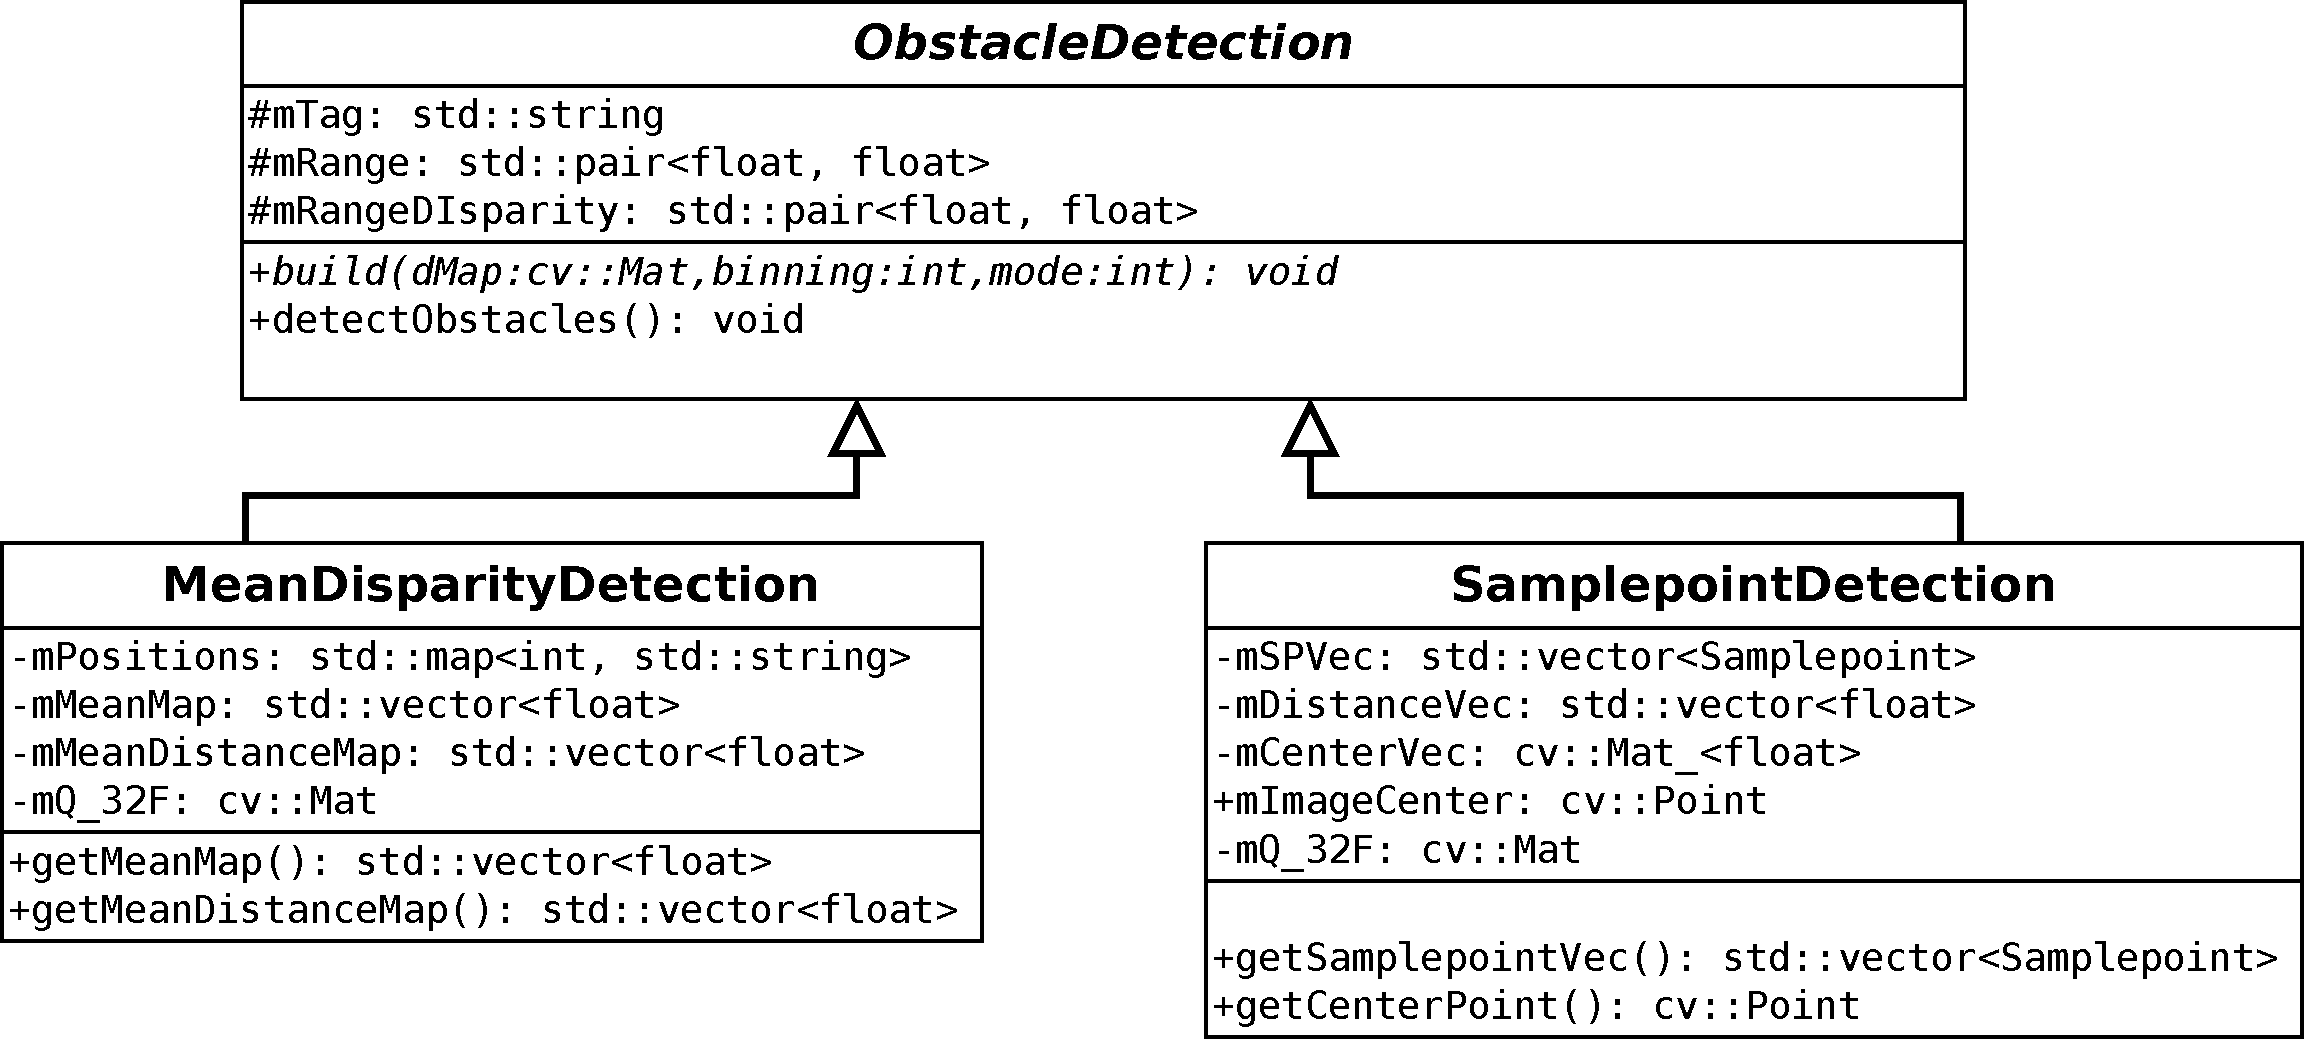
\includegraphics[width=13cm]{img/obstacle_detection_structure.pdf}
%	\end{center}
%	\caption{Klassenstruktur der Hinderniserkennung}
%	\label{fig:obstacle_detection_structure}
%\end{figure}

% ---------------------- section -----------------------
\section{Preprocessing}
\label{sec:preprocessing}
Der Ablauf der Hinderniserkennung ist in beiden entwickelten Methoden gleichbleibend. Die dafür benötigen Preprocessing Schritte gleichen sich demnach ebenfalls und werden im folgenden erläutert.\\

\noindent
\textbf{Region of Interest der Disparity Map:}\\
Zu Beginn des Algorithmus muss der durch die Baseline verursachte nicht matchbare Bereich entfernt werden. Dies geschieht nach der Wahl der in(REF) beschriebenen Parameter der SGBM. Dieser sogenannte Pixelshift berechnet sich aus der Hälfte der Anzahl der zu berechnenden Disparitäten. Sollte dieser einen ungeraden Wert ergeben so wird er um 1 erhöht. Generell ist der Pixelshift so gewählt das die Dimensionen der Disparity Map durch 8 Teilbar sind. Dieser Wert hat sich während der Entwicklung als robuster Wert erwiesen. Weiterhin dient es zur späteren Verteilung der Samplepoints.\\

	% pixelschift durch numdispt/2 bestimmt
	% sofern dieser ungerade 1 addiert zur weiteren vorgehensweise
	% horizontaler pixelshift so gewählt das die dimensionen der disparity map durch 8 teilbar bleiben
	% dies hat sich während der entwicklung als robuster und zuverlässiger wert erwiesen.
	% TODO roi der disparity map
	
\noindent
\textbf{Berechnung der Disparität aus gegebener Distanz:}\\
Um die Algorithmen ressourcensparend zu gestalten wird während der Erkennung mit den reinen Disparitäten gearbeitet. Da die Disparitäten in Abhängigkeit der Bildgröße sowie der Q-Matrix berechnet werden ergibt kann kein fest definierter Disparitätenwert für eine Distanz bestimmt werden. Für diesen Prozess wird die in Anschnitt \ref{sec:framework} beschriebene Distanzberechnung invertiert. Mithilfe der in Formel \ref{eq:backward_calculation} dargestellten Berechnung können nun die jeweilige Position sowie die dazugehörige Disparität berechnet werden. 

\begin{equation}
  \label{eq:backward_calculation}
  \begin{aligned}
    d &= \frac{f- Z' \cdot b}{Z' \cdot a}\\
    I_x &= X' \cdot (d \cdot a + b) + C_x\\
    I_y &= Y' \cdot (d \cdot a + b) + C_y
  \end{aligned}
\end{equation}

\noindent
Dieser Prozess findet in der späteren Initialisierung der Algorithmen Verwendung bei welcher die metrischen Angaben der Erkennungsreichweite in Disparitäten zurückgerechnet werden. Als Referenz wir dazu die Position des Bildhauptpunktes berechnet welcher sich im Ursprung des Weltkoordinatensystems befindet. Diese Vorgehensweise spart in der späteren Hinderniserkennung Ressourcen, da nicht für jedes Subimage bzw. jeden Samplepoint die Weltkoordinate berechnet werden muss. Stattdessen können die Disparitäten direkt verglichen werden. Dies ist in beiden Algorithmen derselbe Schritt.\\

% TODO invertierung distanz zu disparität
	% um ressourcenschonend zu arbeiten wird nicht mit distanzen gearbeitet sondern mit disparitäten
	% daher wichtig zu wissen welche disparität der distanz der range entspricht
	% dafuer wird die in REF beschriebene distanzberechnung invertiert
	% mithilfe diesre rechnnung --> einzelne Pixel werte der disparuty map berechnen
	% als referenz wird der pricipal point gew¨åhlt welcher sich im falle des benutteen sustems nahezu im bildmittelpunkt befindet
	% RECHNUNG
	% dies vorgehensweise spart rechenkraft da nun nicht fuer djedes erkannte hidnerniss eine distanz berechnet werden muss
	%stattdessen wird einfach der Disparity wert genutzt welcher direkt zur verfugung steht
	% bei beiden algorithmen derselbe schritt

\noindent
\textbf{Pointcloud Erstellung:}\\
Die Ausgabe der Pointclouds erfolgt in Stanfords Polygon File Format (ply). Aufgrund der einfachen Struktur können die einzelnen Pointclouds erkannter Hindernisse einfach analysiert werden um etwaige Vermeidungsstrategien zu entwickeln. Weiterhin ermöglicht das ply Format die Visualisierung jedes Frames in denen Hindernisse erkannt wurden.

% TODO pointcloud erstellung generell
	% ausgabe der pcl erfolt im stanford ply format
	% somit können erkannte hindernisse leicht wieder eingelesen werden um vermeidungsstrategien zu entwickeln
	% andereseits können fur jeden frame (in dem ein hindernis vorlag) pointclouds dargestellt werden um etwaige fehler zu erkmitteln
	
%	 Das Format der Ausgabe entspricht dabei Stanford's Polygon File Format ($.ply$). Was die Informationsweitergabe and spätere Module vereinfacht, da die dreidimensionalen Koordinaten pro Zeile abgespeichert werden. Zudem erleichtert

% ---------------------- section -----------------------
\section{Subimage Detection}
\label{sec:mean_disparity_detection}

Das grundlegende Funktionsprinzip der \emph{Subimage Detection} ist grob an die von Kostavelis et al. vorgestellten Algorithmen angelehnt. Auch bei diesen werden die berechneten Disparity Maps in Segmente eingeteilt von welchen in jedem Frame der Mittelwert errechnet wird.\\

\noindent
Zu Beginn des Algorithmus, nach der vorherigen Bearbeitung der eigentlichen \emph{region of interest}, wird während der Initialisierung die Segmentierung der Disparity Map festgelegt. Dabei wird für jedes Segment ein eigenes Subimage erzeugt. Diese definieren eine \emph{region of interest} (ROI) innerhalb einer Matrix. Subimages selber halten lediglich die Positionsinformationen (obere linke und untere rechte Ecke des definierten Rechtecks), Mittelwert der ROI, die ROI selbst sowie den Mittelpunkt des Rechtecks zur späteren Pointcloud Generierung, wie Abbildung \ref{fig:subimage_class} aufzeigt.

\begin{figure}[h]
	\begin{center}
		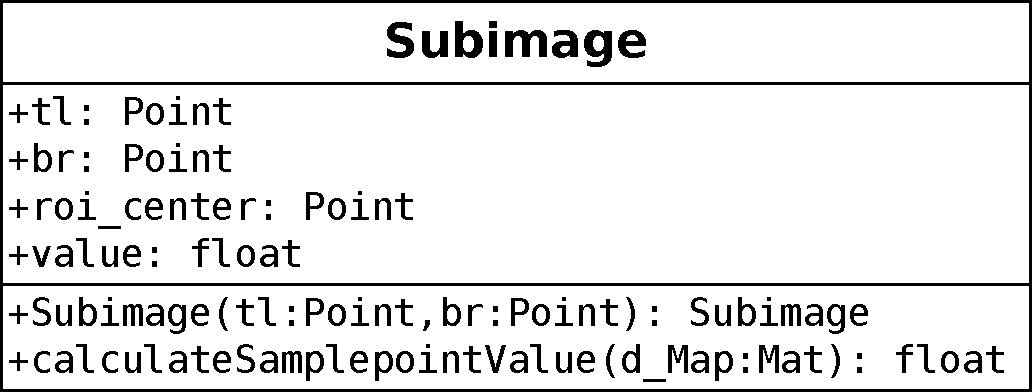
\includegraphics[width=8cm]{img/subimage_class.pdf}
	\end{center}
	\caption{Subimage Klasse}
	\label{fig:subimage_class}
\end{figure}

\noindent
Für die Unterteilung der Disparity Map wurden intial nur $9$ Segmente vorgesehen wobei jeder Bereich eine der möglichen Flugrichtungen repräsentieren sollte. Aufgrund der Größe der Submatrizen konnte jedoch keine valide Erkennung kleiner Hindernisse gewährleistet werden, da solche in der Berechnung des Mittelwertes untergegangen sind. Aufgrund dessen wurde die Anzahl der Segmente auf $81$ erhöht, welches eine wesentlich genauere Erkennung ermöglicht. Zudem ist somit eine weitaus genauere Einteilung der Flugrichtungen möglich, da jede dieser nocheinmal genauer betrachtet wird (siehe Abbildung \ref{fig:subimage_detection_segments}).

\begin{figure}[h]
	\begin{center}
		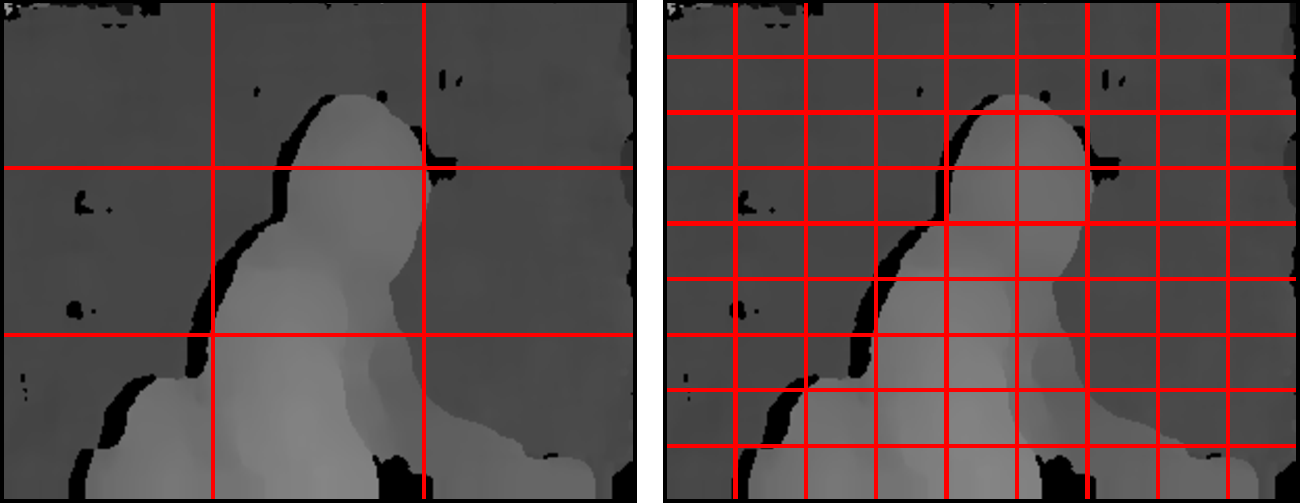
\includegraphics[width=10cm]{img/subimage_segmentation.pdf}
	\end{center}
	\caption{Intiale Segmentierung der Disparity Map sowie die weitere Unterteilung zur genaueren Bestimmung der Werte der Subimages}
	\label{fig:subimage_detection_segments}
\end{figure}

\noindent
Um die Hindernisse innerhalb der Segmente zu Erkennen wurde auf die Berechnung des Mittelwertes dieser gesetzt. Einerseits, da die Berechnung des Mittelwertes unter Betrachtung des Echtzeit-Aspektes eine ressourcensparende und schnelle Operation ist, andererseits weil jeder Pixel des Bildes in das Endresultat mit einfließt. Jedoch musste die Berechnung auf das Szenario angepasst werden, da Berechnung des Medians aller Werte zu Verzerrungen geführt hätte. Bei der Kalkulation von Disparity Maps werden Bereiche welche nicht gematcht werden können, sei es aufgrund von fehlenden Informationen im Referenzbild oder homogener Texturen in der Szene, als negativer Wert ausgedrückt. Berechnet man nun den Mittelwert unter Betrachtung positiver und negativer Werte, so entspricht dies zwar dem definierten Term Median, verfälscht allerdings das in diesem Anwendungsbereich erwünschte Ergebnis. Im schlechtesten Fall enthält eine Submatrix mehr negative als positive Werte, was dazu führen kann das Hindernisse vor homogenen Flächen nicht erkannt werden. Daraus ergibt sich die in Algorithmus \ref{alg:mean_disparity_calculation} dargestellte Berechnung des Mittelwertes.

\begin{algorithm}[h]
\caption{Berechnung des Disparity Medians}
\label{alg:mean_disparity_calculation}
\begin{algorithmic}[1]
    \Procedure{CalcMeanDisparity}{$submatrix$}
        \State $elements_{number} \gets 0$
        \State $elements_{sum} \gets 0 $
        \For{$value$ in $submatrix$}
            \If{$value > 0$}
                \State $elements_{sum} \gets elements_{sum} + value$
                \State $elements_{number} \gets elements_{number} + 1$
            \EndIf
        \EndFor
        \State \textbf{return} $elements_{sum} / elements_{number}$
    \EndProcedure
\end{algorithmic}  
\end{algorithm}

\noindent
Es werden demnach nur positive Disparitäten betrachtet was auch dazu führt das sich der Gesamtwert aller Werte aus der Menge dieser ergibt. Mit Hilfe dieser Berechnung ist es möglich Hindernisse auch in Bereichen zu erkennen in denen die Mehrzahl der Pixel keine Matches aufweisen.\\

\noindent
Die eigentliche Hinderniserkennung erfolgt in jedem Frame. Wobei der Term Frame hierbei nicht nach einem von der Kamera aufgenommenen Bild, sondern eine neue Disparity Map definiert. Da die Bildgröße pro Einzelbild stetig ist besteht keine Nötigkeit die einzelnen Segmente erneut zu generieren. Es genügt also die Mittelwerte eines jeden Subimages anhand der neuen Disparity Map zu aktualisieren. Daraufhin wird geprüft ob sich einer oder mehrere der Subimage Mittelwerte innerhalb der Gefahrenzone befinden. Die Gefahrenzone wird zur Initialisierung der Erkennung berechnet. Mit Hilfe der in Abschnitt \ref{sec:preprocessing} beschriebenen Invertierung der Distanzberechnung müssen zu Beginn die minimale sowie maximale Distanz der Erkennung auf einen Tiefenwert zurückgerechnet werden. Diese Rückrechnung ist ausschlaggebend für die schnelle Erkennung der Tiefe. Im Falle einer weiteren Segmentierung müsste die Berechnung der Distanz als Teil der Weltkoordinate für jedes Subimage einzeln erfolgen, was gerade bei der Samplepoint Detecion zum Tragen kommt, sollen die Distanzen für ca. $6000$ Punkte (bei voller Auflösung in Abhängigkeit der verwendeten Parameter des SGBM) berechnet werden.\\

% TODO subimage detection pseudocode
\begin{algorithm}[h]
\label{alg:mean_disparity_detection}
\begin{algorithmic}[1]
    \Procedure{detectObstacles}{$submatrix$}
		\State $found\_points \gets 0$
		\State $found\_obstacles \gets 0$
		\For{$value$ in $mean\_disparities$}
			\If{$value < range_{min}$ AND $value > range_{max}$}
				\State $temp\_Subimage \gets Subimage\_vector[index_{value}]$
				\State $found\_obstacles \gets found\_obstacles.append(value)$
				\State $coordinate \gets calc\_coordinate(temp\_Subimage$
				\State $found\_points \gets found\_points.append(coordinate)$
			\EndIf
		\EndFor
		\If{$size$ of $found\_points \neq$ $0$}
			\State $write pointcloud for current found_obstacle$
		\EndIf 
    \EndProcedure
\end{algorithmic}
\caption{Ablauf der Hinderniserkennung}
\end{algorithm}

\noindent
Die in Algorithmus \ref{alg:mean_disparity_detection} berechnete Pointcloud ist in diesem Fall ein Matrix mit der Größe der ursprünglichen Tiefenkarte. Dies ist für die Berechnung der dreidimensionalen Koordinate von Nöten. Mithilfe des Mittelpunkte der Subimages wird für jedes dieser die jeweilige 3D-Koordinate (siehe Abschnitt \ref{sec:framework}) berechnet und an der Position des Mittelwertes in die Punktwolke geschrieben.

\noindent
Innerhalb der Pointcloud sind nun die Weltkoordinaten jedes Samplepoints relativ zur Kameraposition gespeichert. Der Vektor zwischen dem Koordinatenursprung und der Koordinate entspricht dabei der Distanz zum Hindernis.

% ---------------------- section -----------------------
\section{Samplepoint Detection}
\label{sec:samplepoint_detection}
In Hinblick auf aktive optische Algorithmen zur 3D-Rekonstruktion und damit verbunden Techniken wir Laser Scanning oder Time of Flight wurde die Samplepoint Detection entwickelt. Das Ziel war dabei eine ressourcensparende Alternative zur Subimage Detection zu schaffen indem nicht zwangsläufig alle Pixel der Disparity Map betrachtet werden müssen.\\

\noindent
Ebenso wie in der in Abschnitt \ref{alg:mean_disparity_calculation} vorgestellten \emph{Subimage Detection} bedient sich die Samplepoint Detection einer vorverarbeiteten Disparity Map zur Hinderniserkennung. Bei der Initialisierung wird die Anzahl der zu berechnenden Samplepoints festgelegt, dabei richtet sich der Wert an der Anzahl der Reihen und Spalten der Disparity Map Matrix um eine äquidistante Verteilung gewährleisten zu können. Der hier verwendete Standart Faktor ist 8 (siehe Formel REF). Dies sorgt unter anderem für eine gleiche Anzahl von Samplepoints im gebinnten und ungebinnten Aufnahmemodus, da die jeweilige Menge relativ zur Bildgröße ist. Auf eine Verteilung der Messpunkte am direkten Rand der Disparity Map wurde bewusst verzichtet, da dieser aufgrund der Rektifizierung eher Fehler aufweist als Bereiche in der Mitte des Bildes.\\

\noindent
Ein Samplepoint umfasst im entwickelten System entweder einen Pixel oder einen Zusammenschluss mehrerer Pixel. Die dabei festgelegte Ausgangskoordinate entspricht dabei entweder dem eigentlichen Punkt, oder dem Mittelpunkt einer festgelegten Region of Interest. Da ein Pixel gerade bei Bildern mit hoher Auflösung weniger Aussagekraft besitzt als der Pixel inklusive der lokalen Umgebung wurde ein Samplepoint auf diese Weise definiert. Der Wert eines einzelnen Samplepoints $S$ mit dem Zentrum $C$ ergibt sich im Falle eines Radius $r=3$ aus dem Mittelwert des Quadrats $Q$ mit den Eckpunkten $Q_{tl} = (C_x - r, C_y -r)$ und $Q_{br} = (C_x + r, C_y +r)$. Dies erhöht zwar die Anzahl der zu betrachtenden Pixel welche jedoch, in Abhängigkeit vom gewählten Radius, geringer ist als die Gesamtzahl aller Bildpunkte. Dieser Prozess wird in Abbildung \ref{fig:samplepoints_initmodes} verdeutlicht.\\

\begin{figure}[h]
	\begin{center}
		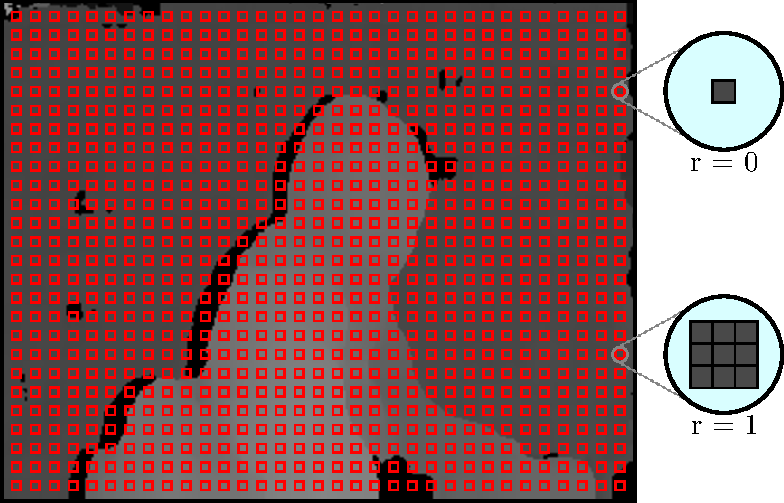
\includegraphics[width=10cm]{img/samplepoints_initmodes.pdf}
	\end{center}
	\caption{Darstellung der Samplepoints mit verschiedenen Radien}
	\label{fig:samplepoints_initmodes}
\end{figure}

\noindent
Nachdem zunächst alle Samplepoints initialisiert wurden, werden die jeweiligen Werte pro Frame aktualisiert. Die eigentliche Erkennung erfolgt dabei einerseits durch die Erstellung einer Pointcloud welche ebenfalls die selben Dimensionen wie die zugrunde liegende Disparity Map besitzt. Erweiternd dazu lässt sich mithilfe der jeweiligen Punkte das als aktuell am gefährlichsten einzustufende Hindernis sowie dessen Position bestimmen. Dabei werden Samplepoints innerhalb der Gefahrenzone zunächst nur auf Bildebene betrachtet.
Zunächst wird die Liste an Samplepoints der errechneten Disparität sortiert.
Da generell Hindernisse direkt vor dem UAV als am kritischsten zu betrachten sind, berechnet der Algorithmus den zweidimensionalen Abstand zwischen Bildhauptpunkt und den Samplepoints mit der geringsten Disparität. 


%------------------------------------------------

\chapter{Konflikte und Lösungsansätze}
\label{chp:conflicts}
In der Erkennung von Hindernissen mithilfe von passiv optischen Systemen können verschiedenste Faktoren der Grund für eine fehlerhafte Erkennung sein. Sei es die Berechnung einer Disparity Map von Bereichen mit einer Vielzahl homogener oder reflektierender Flächen oder die Veränderung der Lichtverhältnisse in einem der beiden Kamerabilder. In diesem Kapitel werden einige der bestehenden, sowie einige potentiell mögliche Fehlerquellen erläutert sowie dazugehörige Lösungsansätze entwickelt.\\

% TODO Zusammenfassung Kapitel

% ---------------------- section -----------------------
\section{Bestehende Konflikte und Lösungsansätze}
\label{sec:existing_conflicts}

Die Validierung der erkannten Hindernisse ist ein kompliziertes Problem in der autonomen Hinderniserkennung. Durch etwaige äußere Einflüsse wie die Veränderung der Lichtverhältnisse kann die Berechnung der Tiefenkarte fehlerhaft sein. Dies kann im Fall eines autonomen Flugs dazu führen, dass das UAV ein Hindernis innerhalb eines Korridors erkennt und aufgrund dessen versucht diesem imaginären Hindernis auszuweichen. Gerade in engen Umgebungen ohne viel verfügbaren Platz kann dies zum totalen Systemausfall führen. Daher sollte ausgewertet werden ob es sich bei erkannten Hindernissen auch um solche handelt. Ein Ansatz zur Vermeidung solcher Falscherkennungen wäre, die Objekte insofern zu verfolgen, dass für jeden Frame (in Abhängigkeit der zugrundeliegenden Framerate) überprüft wird ob bereits im vorherigen Frame ein Objekt gefunden wurde. Erst nachdem dies sichergestellt wurde wird daraufhin eine Warnung ausgegeben. Zeitgleich wäre es möglich, dass Informationen wie die Eigenbewegung sowie die Information ob sich das erkannte Objekt selber im Raum bewegt verloren gehen.\\

\noindent
Eine andere Problematik stellt die Erkennung von homogenen, spiegelnden sowie durchsichtigen Flächen dar. Aufgrund fehlender Texturen sowie vorhandener Pixeldifferenzen kann die Korrespondenz zweier Pixel unter Umständen nicht bestimmt werden. Diese homogenen Bereiche haben demnach fehlerhafte Informationen zur Folge, so kann  einerseits einem Pixel an einer weißen Wand kein zugehöriger Pixel zugeordnet werden, andererseits ist es auch möglich das falsche Bildpunkte miteinander gematcht werden, welche wiederum eine hohe Disparität zur Folge haben. In diesem Fall wird ein Hindernis erkannt obwohl sich keines an dieser Position befunden hat. Abbildung \ref{fig:disparity-error-homogeneous} zeigt deutlich in welchen Bereichen der \emph{SGBM} aufgrund fehlender Textur keine Korrespondenzen finden konnte.\\

\begin{figure}[h]
	\centering
	\begin{tabular}{m{6.5cm} m{6.5cm}}
	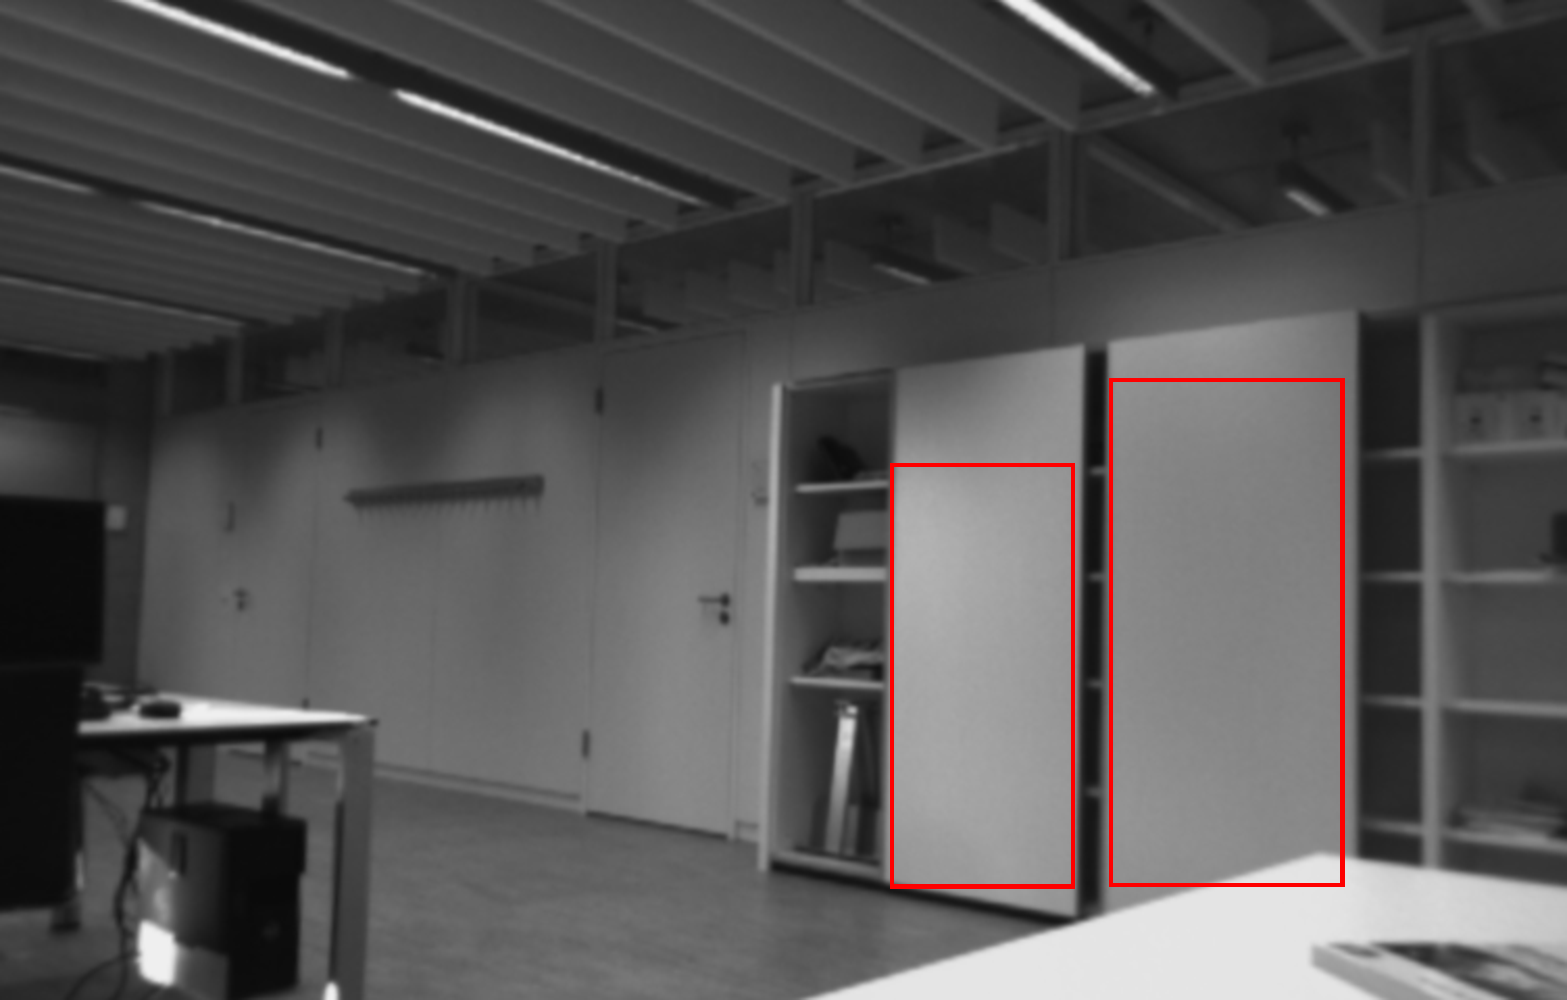
\includegraphics[width=6.5cm]{img/disparity_error_left.pdf}
%	\begin{center} \small (a) linkes Kamerabild \end{center}
	&
	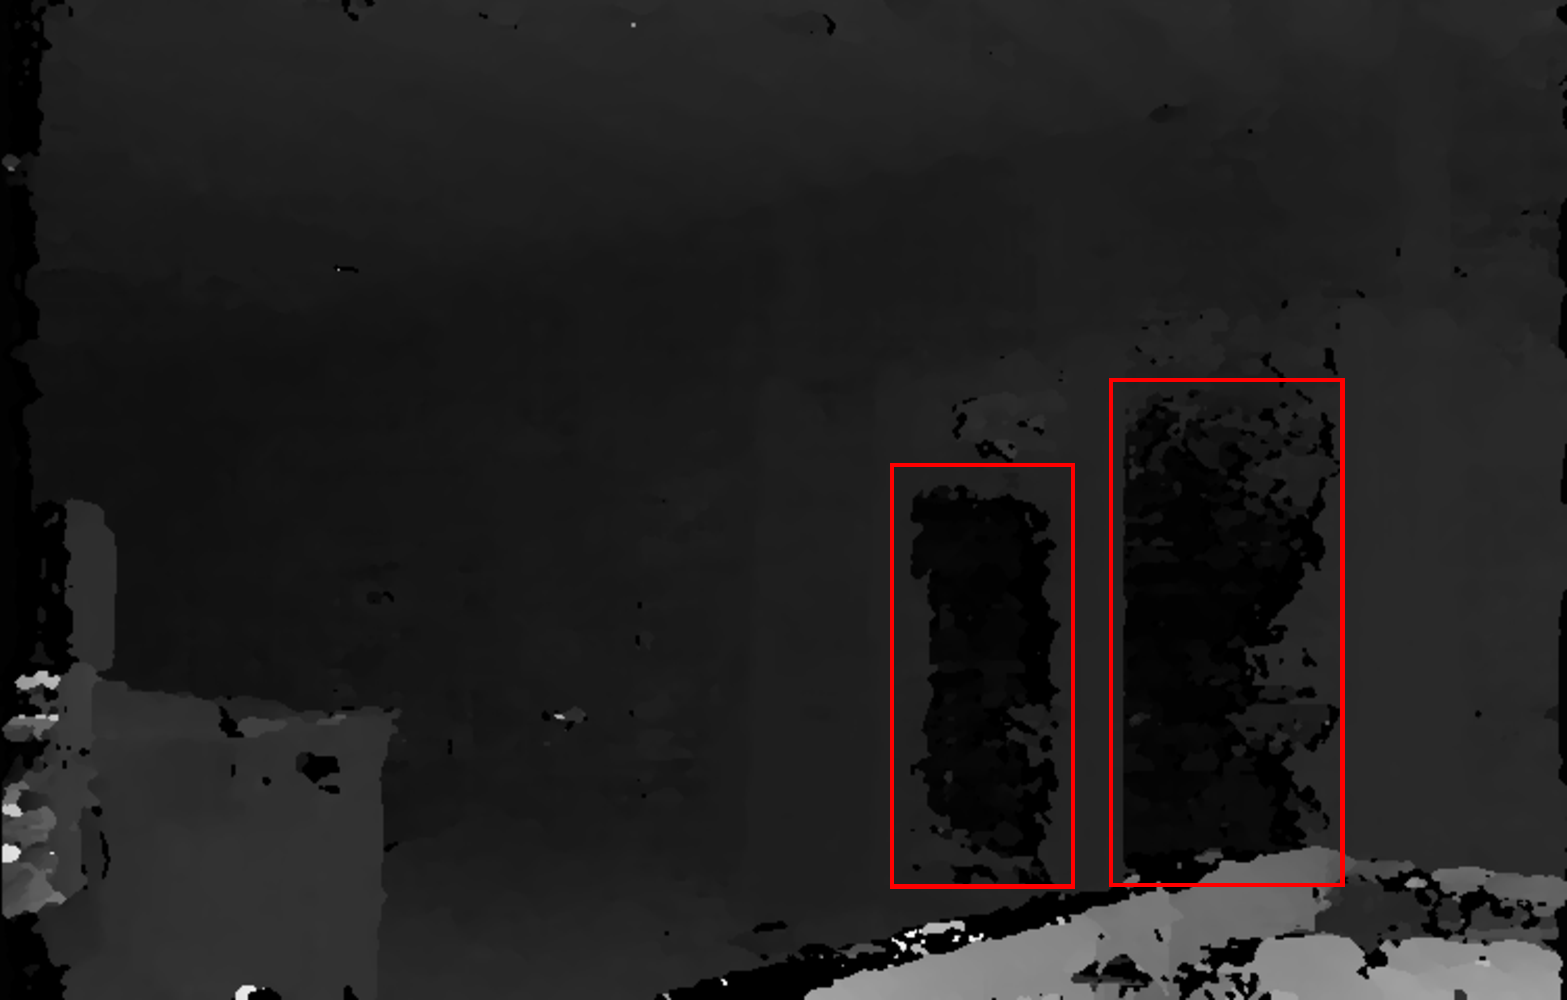
\includegraphics[width=6.5cm]{img/disparity_error.pdf}
%	\begin{center} \small (b) Disparity Map \end{center}
	\end{tabular}
\caption{Konflikt in der Berechnung der Disparität bei nicht texturierten Flächen. Dabei ist (a) das linke aufgenommene Kamerabild und (b) die dazu gehörige Disparity Map. Die in rot markierten Flächen sind das Resultat homogener Texturen.}
\label{fig:disparity-error-homogeneous}
\end{figure}

\noindent
Auch spiegelnde Flächen sind eine optische Problemstellung. Aufgrund der Projektion eines anderen Bereiches kommt es zu falschen Informationen innerhalb der Disparity Map. Hindernisse können zwar erkannt werden sofern sich die spiegelnde Fläche in einer günstigen Position befindet. Dies ist der Fall, wenn beide Kameras exakt den selben Bereich erfassen. Jedoch wird auch in diesem Fall eine weiter entfernte Distanz wahrgenommen anstelle des eigentlichen Objektes. Ist dies nicht der Fall so kann auch im Fall spiegelnder Flächen keine Disparität und folglich keine Tiefe wahrgenommen werden.\\
    % TODO Grafik spiegelnde Flächen
\noindent
Eine weitere Fehlerquelle sind durchsichtige Bereiche. Diese vereinen zum einen Fehlerquellen welche auch bei spiegelnden Arealen auftreten, zum anderen werden Objekte die sich hinter einer Glasscheibe befinden zwar erkannt (sofern keine Reflexion vorliegt) jedoch das Glas als eigentliches Hindernis nicht. Weiterhin besteht die Möglichkeit, dass Reflexionen aus Perspektive der beiden Kameras betrachtet einen anderen Tiefeneindruck vermitteln. Objekte werden so entweder weiter entfernt oder auch in kürzerer Distanz erkannt als sie sich wirklich befinden.\\

\noindent
Aufgrund des Aspektes, dass die Erkennung des Systems auf den Gebrauch in Innenbereichen konzipiert ist, gibt es verschiedenste Probleme bei der Anwendung in Außenbereichen. Zum einen ist die Verschlusszeit der Kameras fixiert. Die Verwendung einer automatischen Belichtungszeit ist nur für jede Kamera einzeln möglich. Um mit verschiedenen Lichtverhältnissen umgehen zu können, ohne dabei die Möglichkeit der Korrespondenzanalyse zu verlieren, muss die Verschlusszeit daher bei beiden Kameras immer gleich sein. Weiterhin ist die Erkennung des Bodens ein zu betrachtender Aspekt. Dieser ist bei aktueller Berechnung ein Teil der zu betrachtenden Hindernisse, was einerseits seine Berechtigung hat, andererseits auch bei niedrigen Flughöhen zu einer fehlerhaften Erkennung als Hindernis führt.
	% TODO Hindernisgröße einbauen


% ---------------------- section -----------------------
\section{Diskussion}
\label{sec:conflict_discussion}
Ein Ansatz erkannte Hindernisse zu validieren ist, sich auf die letzte bekannte Position des Objektes zu berufen und im nächsten Einzelbild zu überprüfen ob es sich noch immer an selber Stelle befindet. Dabei würde für jedes Subimage/ jeden Samplepoint ausgewertet werden ob sich das Hindernis noch innerhalb dessen befindet. Jedoch schränkt dies die Erkennung bewegter Objekte stark ein. Ist die Geschwindigkeit eines Hindernisses so hoch, das in mindestens zwei aufeinanderfolgenden Frames kein Objekt im selben Subimage/Samplepoint erkannt werden kann so würde das System kein Hindernis erkennen können. Diese Methode ist daher prinzipiell mögliche jedoch stark von der Framerate sowie der eigenen bzw. Bewegung des Objektes abhängig. Grundlegend ist das System aufgrund der Beschaffenheit der Subimages für die Mean Disparity Detection geeignet, da die Größe der Subimages eine solche Validierung zulassen würde. Im Falle der Samplepoint Detection müssten auch die unmittelbar benachbarten Messpunkte mit einbezogen werden sodass die Bewegung auch verfolgt werden kann. Eine Kombination von Feature Tracking wäre dabei hilfreich, jedoch sehr rechenaufwändig.\\
    % paper suchen

\noindent
Um auch die Erkennung homogener Flächen gewährleisten zu können besteht die Möglichkeit die Szene mithilfe externer Lichtquellen auszuleuchten um eine Texturierung zu erzwingen. Mit Hilfe eines Lasers würde dabei ein zufälliges Punktmuster auf die Szene projiziert werden, durch welches es dem Matching Algorithmus möglich ist korrespondierende Punkte innerhalb eines nicht texturierten Bereiches zu finden. Die Zufälligkeit der Punktwolke ist dabei ein wichtiges Kriterium, da die Gleichmässigkeit eines Rasters zu falschen Korrespondenzen führen könnte. Die Anwendung dieses Verfahrens ist jedoch hauptsächlich in Innenbereichen möglich, da die zu erkennenden Entfernungen unter Betrachtung der Einzelbild-Auflösung eine Detektion dieser zulassen würden. In Aussenbereichen ist es prinzipiell schwer Hindernisse aufgrund anderer Lichtverhältnisse ausfindig zu machen. Für diesen Anwendungsfall würde sich eine Berechnung homogener Flächen auf Matching Ebene anbieten.

\noindent
In vielen Fällen sind gefundene Stereo Korrespondenzen nicht eindeutig, so beschreiben Geiger et al. \cite{geiger2011efficient} die Berechnung solcher im ELAS (Efficient Large-scale Stereo) Algorithmus. Zu Beginn des Matching Verfahrens wird eine karge Menge an Hilfspunkten berechnet. Diese sind dabei als Pixel definiert welche aufgrund der gegebenen Textur oder ihrer Einzigartigkeit robust gematcht werden können. Dabei werden solche \"Support Points\" als eine Kon­ka­te­na­ti­on der Koordinaten des Pixels $(x_m,v_m) \in \N^2$ sowie der zugehörigen Disparität $d_m \in \N$ definiert. Die Verteilung der Hilfspunkte auf den Referenzbildern erfolgt in gleichem Abstand zueinander. Unklare Matches werden währenddessen anhand eines Thresholds aussortiert. Anschliessend wird unter Zuhilfenahme der erstellten Hilfspunkte nach sogenannten \emph{Observations} gesucht, welche aus den Bildkoordinaten $(x_n,y_n) \in \N^2$ sowie einem Feature Vector $f_n \in \mathfrak{R}^Q$ bestehen. Der Feature Vektor ist dabei entweder die Intensität des Pixels oder ein berechneter Deskriptor, der aus den Intensitäten der benachbarten Pixel berechnet wird. Mithilfe dieser beiden Informationen wird ein Gitternetz generiert. Die eigentliche Berechnung der Disparität erfolgt mit Hilfe der Observations auf deren jeweiliger Epipolarlinie unter Benutzung des Maximum a posteriori (MAP) Verfahrens und wird für jedes Bild separat angewandt. Zuletzt werden beide Disparity Maps auf ihre Konsistenz geprüft.

\noindent
% spiegelnd und reflektierend
Der von Tsin et al. \cite{tsin2003stereo} entwickelte Stereo Matching Algorithmus kann sowohl zwischen Reflexion als auch Transparenz unterscheiden. Dabei wird das grundlegende Problem wie folgt beschrieben: Aufgrund des Reflexionsmodells nach Hero (Abbildung \ref{fig:reflection}(a)) welches besagt das sich Einfalls- sowie Ausfallswinkel, gemessen an der Oberflächennormale gleichen, ist es trivial, dass die Position einer reflexion eines Szenepunkes unabhängig vom aktuellen Sichtfenster ist, da sich die Reflexion an einer festen Position hinter dem Reflektor befindet. Daher kann die Abhängigkeit eines Szenepunktes von seiner Reflexion ignoriert werden. Tsin et al. beschreiben ein geschichtetes Modell in dem das reflektierende Objekt als vordere Ebene $I_0$ und die Reflexion selber als hintere Ebene $I_1$ dargestellt ist (Abbildung \ref{fig:reflection}(b)).\\
% TODO vielleicht grafik noch beschreiben

\begin{figure}[h]
  	\centering
	\begin{tabular}{m{6.5cm} m{6.5cm}}
	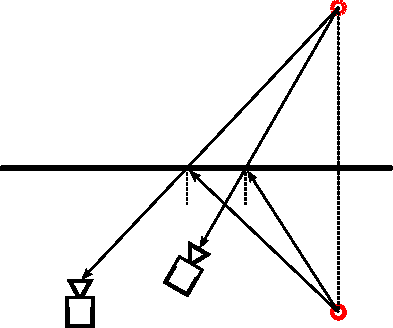
\includegraphics[width=6.5cm]{img/reflection_model_hero.pdf}
	\begin{center} \small (a) \end{center}
	&
	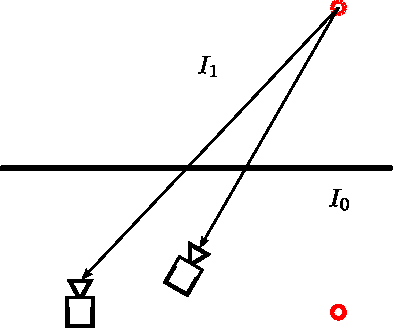
\includegraphics[width=6.5cm]{img/reflection_model_layers.pdf}
	\begin{center} \small (b) \end{center}
	\end{tabular}
\caption{}
\label{fig:reflection}
\end{figure}
%TODO add caption

\noindent
Die Aufgenommenen Bilder sind demnach eine Zusammensetzung beider Ebenen. Selbiges gilt für nicht planare Flächen sowie Durchsichtigkeit solange die Translation zwischen den einzelnen Bildern gering ist. Während des Algorithmus werden die relativen Bewegungen der Ebenen zwischen aufeinanderfolgenden Frames anhand der verschiedenen Tiefen analysiert.


% Hindernisgroesse: ...meh
% aussenbereiche: autofokus meh,
\noindent
Ein weiterer bereits in Abschnitt \ref{sec:existing_conflicts} angeschnittener Punkt ist die Erkennung des Bodens als Hindernis. Dabei stellt sich die Frage ob eine Erkennung als Hindernis gewünscht ist oder nicht. Im Falle einer geringen Flughöhe wird der Boden ebenfalls als Hindernis erkannt. Dies kann einerseits eine Absicherung sein das die durch interne Sensoren ermittelte Flughöhe korrekt ist, andrerseits kann es dazu führen, dass der Algorithmus zur Vermeidung von Hindernissen versucht dieses zu  umgehen. Dies könnte unter Umständen dazu führen, dass das UAV eine Flughöhe annimmt welche über der, durch die Umgebung gegebenen, maximalen Flughöhe liegt. Eine mögliche Lösung wäre die Erkennung des Bodens in Abhängigkeit der aktuellen Höhe zu gestalten. Sollte sich das UAV unter der zur Erkennung des Bodens nötigen Flughöhe befinden so wird diese deaktiviert und der Boden wird nicht weiter betrachtet. Sofern die Flughöhe die Erkennung des Bodens ausschließt wird dieser entfernt.


%------------------------------------------------

\chapter{Evaluierung}
\label{chp:evaluation}
% ---------------------- section -----------------------
\section{Aufbau des Testsetups}
\label{sec:aufbau}

% ---------------------- section -----------------------
\section{Evaluierung Subimage Detection}
\label{sec:evaluierung_subimage}

    \subsection{Robustheit}
    \label{subsec:subimage_robustheit}

    \subsection{Performanz}
    \label{subsec:subimage_performanz}

% ---------------------- section -----------------------
\section{Evaluierung Samplepoint Detection}
\label{sec:evaluierung_samplepoint}

    \subsection{Robustheit}
    \label{subsec:samplepoint_robustheit}    

    \subsection{Performanz}
    \label{subsec:samplepoint_performanz}

%------------------------------------------------

\chapter{Diskussion}
\label{chp:discussion}
% ---------------------- section -----------------------
\section{Ergebnisse der Evaluation}
\label{sec:anforderunsevaluierung}

% generell ist zu sagen das die mean besser funktioniert wenn die hindernisse nicht vor einem weit entfernten hintergrund platziert werden
% durch die geringen disparitäten der hinteren 'ebene' wirrd der median so weit verzerrt, dass kleine objekte einfach nicht mehr auffallen
% wenn hintergrund höhere disparitäten aufweist fallen hohe disparitäten auch mehr ins gewicht

% ---------------------- section -----------------------
\section{Gegenüberstellung beider Algorithmen}
\label{sec:gegenueberstellung}

\subsection{Robustheit}
\label{subsec:discussion_robsutness}
	
	% bisschen mehr statistik kram
	% welcher ist wo signifikant besser
		% bezug auf hindernisgroesse
		% wahrscheinlichkeit das hindernis schlecht uz erkennen aber trotzdem wird es erkannt

\subsection{Performance}
\label{subsec:discussion_performance}
  
    % hinsichtlich performance verschiedene Punkte betrachtet
    % erkennung pro frame im mittel
    % framerate der Disparity berechnung
    % gesamte framerate und ausblick auf die darurch erreichbare performance
    % evtl auslagern und eigenne section machen da beide direkt gegenübergestllt werden können.



%------------------------------------------------

\chapter{Fazit und zukünftige Arbeiten}
\label{chp:fazit}
Im Rahmen dieser Arbeit wurden zwei Methoden zur Erkennung von Hindernissen in Echtzeit entwickelt. Die grundlegende Funktionsweise beider Methoden unterscheidet sich nur in der Verwendung ihrer zugrundeliegenden Datenstruktur. Trotzdessen ist im Lauf der Entwicklung ein deutlicher Unterschied in der Robustheit sowie der Performance zu erkennen gewesen. In zukünftigen Arbeiten sollten beide Methoden in realen Szenarien getestet werden.\\

\noindent
Die während der Evaluation erhaltenen Daten deuten auf eine robuste Funktionsweise beider Methoden hin. Die getestete Performance ist, gerade bei zusätzlich skalierten Bildern so gut, dass prinzipiell auch Echtzeitanwendungen bei hoher Geschwindigkeit denkbar sind. Weiterhin erlaubt gerade die hohe Performance zusätzliche Berechnungen zur Verbesserung der Hinderniserkennung.\\

\noindent
Zur Verbesserung der Ergebnisse ist zudem die Entwicklung eines eigenen Algorithmus zur Berechnung der Disparitätenkarte denkbar. Dieser sollte sowohl schnelle als auch robuste Ergebnisse liefern, wobei die visuelle Qualität nicht die oberste Priorität ist. Eine Parallelisierung dessen ist dabei zur Verbesserung der Performance überlegenswert.\\

\noindent
Weiterhin ist die Integration des entwickelten Systems in einen ROS Node zur weitergehenden Verwendung durch SLAM Algorithmen ein wichtiger Bestandteil zukünftiger Arbeiten. Damit verbunden ist gleichzeitig die Entwicklung eines Systems zur Hindernisvermeidung unter Verwendung der erstellten Punktwolken. In Kombination mit der aktuellen Position sowie Rotation der Drohne im Raum ist die darauffolgende Kartographierung gefundener Hindernisse möglich.\\

\noindent



% performance sehr gut
% nicht parallelisiert --> einerseits genug raum fuer SLAM algorithmen oä, andererseits weniger performance in der hinderniserkennung jedoch gut daher wahrscheinlich egal

% erkennung kleiner hindernissc im binning mode muss verbessert werden oder performance des ungebinnten höher
% implementierung in ros node weiterleitung der ergebnisse mithilfe von messages kp wie das geht
% limitierungen klären
% eigener disparity algorithmus welcher evll nur fuer diesen gebrauch ausgelegt ist

% future, stddev zur bestimmung der hindernis priorität auf alle erkannten Hindernisse angewandt


%------------------------------------------------
%	APPENDIX
%------------------------------------------------

\appendix

%------------------------------------------------
%	IMAGES APPENDIX
%------------------------------------------------

%\listoffigures

%------------------------------------------------
%	TABLES APPENDIX
%------------------------------------------------

%\listoftables

%------------------------------------------------
%	REFERENCES
%------------------------------------------------

\bibliographystyle{apalike}    
\bibliography{main_bib.bib}

% book sources
\nocite{zureiki2008stereo}
\nocite{opencvoreilly}
\nocite{cyganek2011introduction}

%------------------------------------------------
%	END OF DOCUMENT
%------------------------------------------------

\end{document}